\documentclass[11pt]{article}

    \usepackage[breakable]{tcolorbox}
    \usepackage{parskip} % Stop auto-indenting (to mimic markdown behaviour)
    
    \usepackage{iftex}
    \ifPDFTeX
    	\usepackage[T1]{fontenc}
    	\usepackage{mathpazo}
    \else
    	\usepackage{fontspec}
    \fi

    % Basic figure setup, for now with no caption control since it's done
    % automatically by Pandoc (which extracts ![](path) syntax from Markdown).
    \usepackage{graphicx}
    % Maintain compatibility with old templates. Remove in nbconvert 6.0
    \let\Oldincludegraphics\includegraphics
    % Ensure that by default, figures have no caption (until we provide a
    % proper Figure object with a Caption API and a way to capture that
    % in the conversion process - todo).
    \usepackage{caption}
    \DeclareCaptionFormat{nocaption}{}
    \captionsetup{format=nocaption,aboveskip=0pt,belowskip=0pt}

    \usepackage[Export]{adjustbox} % Used to constrain images to a maximum size
    \adjustboxset{max size={0.9\linewidth}{0.9\paperheight}}
    \usepackage{float}
    \floatplacement{figure}{H} % forces figures to be placed at the correct location
    \usepackage{xcolor} % Allow colors to be defined
    \usepackage{enumerate} % Needed for markdown enumerations to work
    \usepackage{geometry} % Used to adjust the document margins
    \usepackage{amsmath} % Equations
    \usepackage{amssymb} % Equations
    \usepackage{textcomp} % defines textquotesingle
    % Hack from http://tex.stackexchange.com/a/47451/13684:
    \AtBeginDocument{%
        \def\PYZsq{\textquotesingle}% Upright quotes in Pygmentized code
    }
    \usepackage{upquote} % Upright quotes for verbatim code
    \usepackage{eurosym} % defines \euro
    \usepackage[mathletters]{ucs} % Extended unicode (utf-8) support
    \usepackage{fancyvrb} % verbatim replacement that allows latex
    \usepackage{grffile} % extends the file name processing of package graphics 
                         % to support a larger range
    \makeatletter % fix for grffile with XeLaTeX
    \def\Gread@@xetex#1{%
      \IfFileExists{"\Gin@base".bb}%
      {\Gread@eps{\Gin@base.bb}}%
      {\Gread@@xetex@aux#1}%
    }
    \makeatother

    % The hyperref package gives us a pdf with properly built
    % internal navigation ('pdf bookmarks' for the table of contents,
    % internal cross-reference links, web links for URLs, etc.)
    \usepackage{hyperref}
    % The default LaTeX title has an obnoxious amount of whitespace. By default,
    % titling removes some of it. It also provides customization options.
    \usepackage{titling}
    \usepackage{longtable} % longtable support required by pandoc >1.10
    \usepackage{booktabs}  % table support for pandoc > 1.12.2
    \usepackage[inline]{enumitem} % IRkernel/repr support (it uses the enumerate* environment)
    \usepackage[normalem]{ulem} % ulem is needed to support strikethroughs (\sout)
                                % normalem makes italics be italics, not underlines
    \usepackage{mathrsfs}
    

    
    % Colors for the hyperref package
    \definecolor{urlcolor}{rgb}{0,.145,.698}
    \definecolor{linkcolor}{rgb}{.71,0.21,0.01}
    \definecolor{citecolor}{rgb}{.12,.54,.11}

    % ANSI colors
    \definecolor{ansi-black}{HTML}{3E424D}
    \definecolor{ansi-black-intense}{HTML}{282C36}
    \definecolor{ansi-red}{HTML}{E75C58}
    \definecolor{ansi-red-intense}{HTML}{B22B31}
    \definecolor{ansi-green}{HTML}{00A250}
    \definecolor{ansi-green-intense}{HTML}{007427}
    \definecolor{ansi-yellow}{HTML}{DDB62B}
    \definecolor{ansi-yellow-intense}{HTML}{B27D12}
    \definecolor{ansi-blue}{HTML}{208FFB}
    \definecolor{ansi-blue-intense}{HTML}{0065CA}
    \definecolor{ansi-magenta}{HTML}{D160C4}
    \definecolor{ansi-magenta-intense}{HTML}{A03196}
    \definecolor{ansi-cyan}{HTML}{60C6C8}
    \definecolor{ansi-cyan-intense}{HTML}{258F8F}
    \definecolor{ansi-white}{HTML}{C5C1B4}
    \definecolor{ansi-white-intense}{HTML}{A1A6B2}
    \definecolor{ansi-default-inverse-fg}{HTML}{FFFFFF}
    \definecolor{ansi-default-inverse-bg}{HTML}{000000}

    % commands and environments needed by pandoc snippets
    % extracted from the output of `pandoc -s`
    \providecommand{\tightlist}{%
      \setlength{\itemsep}{0pt}\setlength{\parskip}{0pt}}
    \DefineVerbatimEnvironment{Highlighting}{Verbatim}{commandchars=\\\{\}}
    % Add ',fontsize=\small' for more characters per line
    \newenvironment{Shaded}{}{}
    \newcommand{\KeywordTok}[1]{\textcolor[rgb]{0.00,0.44,0.13}{\textbf{{#1}}}}
    \newcommand{\DataTypeTok}[1]{\textcolor[rgb]{0.56,0.13,0.00}{{#1}}}
    \newcommand{\DecValTok}[1]{\textcolor[rgb]{0.25,0.63,0.44}{{#1}}}
    \newcommand{\BaseNTok}[1]{\textcolor[rgb]{0.25,0.63,0.44}{{#1}}}
    \newcommand{\FloatTok}[1]{\textcolor[rgb]{0.25,0.63,0.44}{{#1}}}
    \newcommand{\CharTok}[1]{\textcolor[rgb]{0.25,0.44,0.63}{{#1}}}
    \newcommand{\StringTok}[1]{\textcolor[rgb]{0.25,0.44,0.63}{{#1}}}
    \newcommand{\CommentTok}[1]{\textcolor[rgb]{0.38,0.63,0.69}{\textit{{#1}}}}
    \newcommand{\OtherTok}[1]{\textcolor[rgb]{0.00,0.44,0.13}{{#1}}}
    \newcommand{\AlertTok}[1]{\textcolor[rgb]{1.00,0.00,0.00}{\textbf{{#1}}}}
    \newcommand{\FunctionTok}[1]{\textcolor[rgb]{0.02,0.16,0.49}{{#1}}}
    \newcommand{\RegionMarkerTok}[1]{{#1}}
    \newcommand{\ErrorTok}[1]{\textcolor[rgb]{1.00,0.00,0.00}{\textbf{{#1}}}}
    \newcommand{\NormalTok}[1]{{#1}}
    
    % Additional commands for more recent versions of Pandoc
    \newcommand{\ConstantTok}[1]{\textcolor[rgb]{0.53,0.00,0.00}{{#1}}}
    \newcommand{\SpecialCharTok}[1]{\textcolor[rgb]{0.25,0.44,0.63}{{#1}}}
    \newcommand{\VerbatimStringTok}[1]{\textcolor[rgb]{0.25,0.44,0.63}{{#1}}}
    \newcommand{\SpecialStringTok}[1]{\textcolor[rgb]{0.73,0.40,0.53}{{#1}}}
    \newcommand{\ImportTok}[1]{{#1}}
    \newcommand{\DocumentationTok}[1]{\textcolor[rgb]{0.73,0.13,0.13}{\textit{{#1}}}}
    \newcommand{\AnnotationTok}[1]{\textcolor[rgb]{0.38,0.63,0.69}{\textbf{\textit{{#1}}}}}
    \newcommand{\CommentVarTok}[1]{\textcolor[rgb]{0.38,0.63,0.69}{\textbf{\textit{{#1}}}}}
    \newcommand{\VariableTok}[1]{\textcolor[rgb]{0.10,0.09,0.49}{{#1}}}
    \newcommand{\ControlFlowTok}[1]{\textcolor[rgb]{0.00,0.44,0.13}{\textbf{{#1}}}}
    \newcommand{\OperatorTok}[1]{\textcolor[rgb]{0.40,0.40,0.40}{{#1}}}
    \newcommand{\BuiltInTok}[1]{{#1}}
    \newcommand{\ExtensionTok}[1]{{#1}}
    \newcommand{\PreprocessorTok}[1]{\textcolor[rgb]{0.74,0.48,0.00}{{#1}}}
    \newcommand{\AttributeTok}[1]{\textcolor[rgb]{0.49,0.56,0.16}{{#1}}}
    \newcommand{\InformationTok}[1]{\textcolor[rgb]{0.38,0.63,0.69}{\textbf{\textit{{#1}}}}}
    \newcommand{\WarningTok}[1]{\textcolor[rgb]{0.38,0.63,0.69}{\textbf{\textit{{#1}}}}}
    
    
    % Define a nice break command that doesn't care if a line doesn't already
    % exist.
    \def\br{\hspace*{\fill} \\* }
    % Math Jax compatibility definitions
    \def\gt{>}
    \def\lt{<}
    \let\Oldtex\TeX
    \let\Oldlatex\LaTeX
    \renewcommand{\TeX}{\textrm{\Oldtex}}
    \renewcommand{\LaTeX}{\textrm{\Oldlatex}}
    % Document parameters
    % Document title
    \title{From smox-grains to resistance}
    
    
    
    
    
% Pygments definitions
\makeatletter
\def\PY@reset{\let\PY@it=\relax \let\PY@bf=\relax%
    \let\PY@ul=\relax \let\PY@tc=\relax%
    \let\PY@bc=\relax \let\PY@ff=\relax}
\def\PY@tok#1{\csname PY@tok@#1\endcsname}
\def\PY@toks#1+{\ifx\relax#1\empty\else%
    \PY@tok{#1}\expandafter\PY@toks\fi}
\def\PY@do#1{\PY@bc{\PY@tc{\PY@ul{%
    \PY@it{\PY@bf{\PY@ff{#1}}}}}}}
\def\PY#1#2{\PY@reset\PY@toks#1+\relax+\PY@do{#2}}

\expandafter\def\csname PY@tok@w\endcsname{\def\PY@tc##1{\textcolor[rgb]{0.73,0.73,0.73}{##1}}}
\expandafter\def\csname PY@tok@c\endcsname{\let\PY@it=\textit\def\PY@tc##1{\textcolor[rgb]{0.25,0.50,0.50}{##1}}}
\expandafter\def\csname PY@tok@cp\endcsname{\def\PY@tc##1{\textcolor[rgb]{0.74,0.48,0.00}{##1}}}
\expandafter\def\csname PY@tok@k\endcsname{\let\PY@bf=\textbf\def\PY@tc##1{\textcolor[rgb]{0.00,0.50,0.00}{##1}}}
\expandafter\def\csname PY@tok@kp\endcsname{\def\PY@tc##1{\textcolor[rgb]{0.00,0.50,0.00}{##1}}}
\expandafter\def\csname PY@tok@kt\endcsname{\def\PY@tc##1{\textcolor[rgb]{0.69,0.00,0.25}{##1}}}
\expandafter\def\csname PY@tok@o\endcsname{\def\PY@tc##1{\textcolor[rgb]{0.40,0.40,0.40}{##1}}}
\expandafter\def\csname PY@tok@ow\endcsname{\let\PY@bf=\textbf\def\PY@tc##1{\textcolor[rgb]{0.67,0.13,1.00}{##1}}}
\expandafter\def\csname PY@tok@nb\endcsname{\def\PY@tc##1{\textcolor[rgb]{0.00,0.50,0.00}{##1}}}
\expandafter\def\csname PY@tok@nf\endcsname{\def\PY@tc##1{\textcolor[rgb]{0.00,0.00,1.00}{##1}}}
\expandafter\def\csname PY@tok@nc\endcsname{\let\PY@bf=\textbf\def\PY@tc##1{\textcolor[rgb]{0.00,0.00,1.00}{##1}}}
\expandafter\def\csname PY@tok@nn\endcsname{\let\PY@bf=\textbf\def\PY@tc##1{\textcolor[rgb]{0.00,0.00,1.00}{##1}}}
\expandafter\def\csname PY@tok@ne\endcsname{\let\PY@bf=\textbf\def\PY@tc##1{\textcolor[rgb]{0.82,0.25,0.23}{##1}}}
\expandafter\def\csname PY@tok@nv\endcsname{\def\PY@tc##1{\textcolor[rgb]{0.10,0.09,0.49}{##1}}}
\expandafter\def\csname PY@tok@no\endcsname{\def\PY@tc##1{\textcolor[rgb]{0.53,0.00,0.00}{##1}}}
\expandafter\def\csname PY@tok@nl\endcsname{\def\PY@tc##1{\textcolor[rgb]{0.63,0.63,0.00}{##1}}}
\expandafter\def\csname PY@tok@ni\endcsname{\let\PY@bf=\textbf\def\PY@tc##1{\textcolor[rgb]{0.60,0.60,0.60}{##1}}}
\expandafter\def\csname PY@tok@na\endcsname{\def\PY@tc##1{\textcolor[rgb]{0.49,0.56,0.16}{##1}}}
\expandafter\def\csname PY@tok@nt\endcsname{\let\PY@bf=\textbf\def\PY@tc##1{\textcolor[rgb]{0.00,0.50,0.00}{##1}}}
\expandafter\def\csname PY@tok@nd\endcsname{\def\PY@tc##1{\textcolor[rgb]{0.67,0.13,1.00}{##1}}}
\expandafter\def\csname PY@tok@s\endcsname{\def\PY@tc##1{\textcolor[rgb]{0.73,0.13,0.13}{##1}}}
\expandafter\def\csname PY@tok@sd\endcsname{\let\PY@it=\textit\def\PY@tc##1{\textcolor[rgb]{0.73,0.13,0.13}{##1}}}
\expandafter\def\csname PY@tok@si\endcsname{\let\PY@bf=\textbf\def\PY@tc##1{\textcolor[rgb]{0.73,0.40,0.53}{##1}}}
\expandafter\def\csname PY@tok@se\endcsname{\let\PY@bf=\textbf\def\PY@tc##1{\textcolor[rgb]{0.73,0.40,0.13}{##1}}}
\expandafter\def\csname PY@tok@sr\endcsname{\def\PY@tc##1{\textcolor[rgb]{0.73,0.40,0.53}{##1}}}
\expandafter\def\csname PY@tok@ss\endcsname{\def\PY@tc##1{\textcolor[rgb]{0.10,0.09,0.49}{##1}}}
\expandafter\def\csname PY@tok@sx\endcsname{\def\PY@tc##1{\textcolor[rgb]{0.00,0.50,0.00}{##1}}}
\expandafter\def\csname PY@tok@m\endcsname{\def\PY@tc##1{\textcolor[rgb]{0.40,0.40,0.40}{##1}}}
\expandafter\def\csname PY@tok@gh\endcsname{\let\PY@bf=\textbf\def\PY@tc##1{\textcolor[rgb]{0.00,0.00,0.50}{##1}}}
\expandafter\def\csname PY@tok@gu\endcsname{\let\PY@bf=\textbf\def\PY@tc##1{\textcolor[rgb]{0.50,0.00,0.50}{##1}}}
\expandafter\def\csname PY@tok@gd\endcsname{\def\PY@tc##1{\textcolor[rgb]{0.63,0.00,0.00}{##1}}}
\expandafter\def\csname PY@tok@gi\endcsname{\def\PY@tc##1{\textcolor[rgb]{0.00,0.63,0.00}{##1}}}
\expandafter\def\csname PY@tok@gr\endcsname{\def\PY@tc##1{\textcolor[rgb]{1.00,0.00,0.00}{##1}}}
\expandafter\def\csname PY@tok@ge\endcsname{\let\PY@it=\textit}
\expandafter\def\csname PY@tok@gs\endcsname{\let\PY@bf=\textbf}
\expandafter\def\csname PY@tok@gp\endcsname{\let\PY@bf=\textbf\def\PY@tc##1{\textcolor[rgb]{0.00,0.00,0.50}{##1}}}
\expandafter\def\csname PY@tok@go\endcsname{\def\PY@tc##1{\textcolor[rgb]{0.53,0.53,0.53}{##1}}}
\expandafter\def\csname PY@tok@gt\endcsname{\def\PY@tc##1{\textcolor[rgb]{0.00,0.27,0.87}{##1}}}
\expandafter\def\csname PY@tok@err\endcsname{\def\PY@bc##1{\setlength{\fboxsep}{0pt}\fcolorbox[rgb]{1.00,0.00,0.00}{1,1,1}{\strut ##1}}}
\expandafter\def\csname PY@tok@kc\endcsname{\let\PY@bf=\textbf\def\PY@tc##1{\textcolor[rgb]{0.00,0.50,0.00}{##1}}}
\expandafter\def\csname PY@tok@kd\endcsname{\let\PY@bf=\textbf\def\PY@tc##1{\textcolor[rgb]{0.00,0.50,0.00}{##1}}}
\expandafter\def\csname PY@tok@kn\endcsname{\let\PY@bf=\textbf\def\PY@tc##1{\textcolor[rgb]{0.00,0.50,0.00}{##1}}}
\expandafter\def\csname PY@tok@kr\endcsname{\let\PY@bf=\textbf\def\PY@tc##1{\textcolor[rgb]{0.00,0.50,0.00}{##1}}}
\expandafter\def\csname PY@tok@bp\endcsname{\def\PY@tc##1{\textcolor[rgb]{0.00,0.50,0.00}{##1}}}
\expandafter\def\csname PY@tok@fm\endcsname{\def\PY@tc##1{\textcolor[rgb]{0.00,0.00,1.00}{##1}}}
\expandafter\def\csname PY@tok@vc\endcsname{\def\PY@tc##1{\textcolor[rgb]{0.10,0.09,0.49}{##1}}}
\expandafter\def\csname PY@tok@vg\endcsname{\def\PY@tc##1{\textcolor[rgb]{0.10,0.09,0.49}{##1}}}
\expandafter\def\csname PY@tok@vi\endcsname{\def\PY@tc##1{\textcolor[rgb]{0.10,0.09,0.49}{##1}}}
\expandafter\def\csname PY@tok@vm\endcsname{\def\PY@tc##1{\textcolor[rgb]{0.10,0.09,0.49}{##1}}}
\expandafter\def\csname PY@tok@sa\endcsname{\def\PY@tc##1{\textcolor[rgb]{0.73,0.13,0.13}{##1}}}
\expandafter\def\csname PY@tok@sb\endcsname{\def\PY@tc##1{\textcolor[rgb]{0.73,0.13,0.13}{##1}}}
\expandafter\def\csname PY@tok@sc\endcsname{\def\PY@tc##1{\textcolor[rgb]{0.73,0.13,0.13}{##1}}}
\expandafter\def\csname PY@tok@dl\endcsname{\def\PY@tc##1{\textcolor[rgb]{0.73,0.13,0.13}{##1}}}
\expandafter\def\csname PY@tok@s2\endcsname{\def\PY@tc##1{\textcolor[rgb]{0.73,0.13,0.13}{##1}}}
\expandafter\def\csname PY@tok@sh\endcsname{\def\PY@tc##1{\textcolor[rgb]{0.73,0.13,0.13}{##1}}}
\expandafter\def\csname PY@tok@s1\endcsname{\def\PY@tc##1{\textcolor[rgb]{0.73,0.13,0.13}{##1}}}
\expandafter\def\csname PY@tok@mb\endcsname{\def\PY@tc##1{\textcolor[rgb]{0.40,0.40,0.40}{##1}}}
\expandafter\def\csname PY@tok@mf\endcsname{\def\PY@tc##1{\textcolor[rgb]{0.40,0.40,0.40}{##1}}}
\expandafter\def\csname PY@tok@mh\endcsname{\def\PY@tc##1{\textcolor[rgb]{0.40,0.40,0.40}{##1}}}
\expandafter\def\csname PY@tok@mi\endcsname{\def\PY@tc##1{\textcolor[rgb]{0.40,0.40,0.40}{##1}}}
\expandafter\def\csname PY@tok@il\endcsname{\def\PY@tc##1{\textcolor[rgb]{0.40,0.40,0.40}{##1}}}
\expandafter\def\csname PY@tok@mo\endcsname{\def\PY@tc##1{\textcolor[rgb]{0.40,0.40,0.40}{##1}}}
\expandafter\def\csname PY@tok@ch\endcsname{\let\PY@it=\textit\def\PY@tc##1{\textcolor[rgb]{0.25,0.50,0.50}{##1}}}
\expandafter\def\csname PY@tok@cm\endcsname{\let\PY@it=\textit\def\PY@tc##1{\textcolor[rgb]{0.25,0.50,0.50}{##1}}}
\expandafter\def\csname PY@tok@cpf\endcsname{\let\PY@it=\textit\def\PY@tc##1{\textcolor[rgb]{0.25,0.50,0.50}{##1}}}
\expandafter\def\csname PY@tok@c1\endcsname{\let\PY@it=\textit\def\PY@tc##1{\textcolor[rgb]{0.25,0.50,0.50}{##1}}}
\expandafter\def\csname PY@tok@cs\endcsname{\let\PY@it=\textit\def\PY@tc##1{\textcolor[rgb]{0.25,0.50,0.50}{##1}}}

\def\PYZbs{\char`\\}
\def\PYZus{\char`\_}
\def\PYZob{\char`\{}
\def\PYZcb{\char`\}}
\def\PYZca{\char`\^}
\def\PYZam{\char`\&}
\def\PYZlt{\char`\<}
\def\PYZgt{\char`\>}
\def\PYZsh{\char`\#}
\def\PYZpc{\char`\%}
\def\PYZdl{\char`\$}
\def\PYZhy{\char`\-}
\def\PYZsq{\char`\'}
\def\PYZdq{\char`\"}
\def\PYZti{\char`\~}
% for compatibility with earlier versions
\def\PYZat{@}
\def\PYZlb{[}
\def\PYZrb{]}
\makeatother


    % For linebreaks inside Verbatim environment from package fancyvrb. 
    \makeatletter
        \newbox\Wrappedcontinuationbox 
        \newbox\Wrappedvisiblespacebox 
        \newcommand*\Wrappedvisiblespace {\textcolor{red}{\textvisiblespace}} 
        \newcommand*\Wrappedcontinuationsymbol {\textcolor{red}{\llap{\tiny$\m@th\hookrightarrow$}}} 
        \newcommand*\Wrappedcontinuationindent {3ex } 
        \newcommand*\Wrappedafterbreak {\kern\Wrappedcontinuationindent\copy\Wrappedcontinuationbox} 
        % Take advantage of the already applied Pygments mark-up to insert 
        % potential linebreaks for TeX processing. 
        %        {, <, #, %, $, ' and ": go to next line. 
        %        _, }, ^, &, >, - and ~: stay at end of broken line. 
        % Use of \textquotesingle for straight quote. 
        \newcommand*\Wrappedbreaksatspecials {% 
            \def\PYGZus{\discretionary{\char`\_}{\Wrappedafterbreak}{\char`\_}}% 
            \def\PYGZob{\discretionary{}{\Wrappedafterbreak\char`\{}{\char`\{}}% 
            \def\PYGZcb{\discretionary{\char`\}}{\Wrappedafterbreak}{\char`\}}}% 
            \def\PYGZca{\discretionary{\char`\^}{\Wrappedafterbreak}{\char`\^}}% 
            \def\PYGZam{\discretionary{\char`\&}{\Wrappedafterbreak}{\char`\&}}% 
            \def\PYGZlt{\discretionary{}{\Wrappedafterbreak\char`\<}{\char`\<}}% 
            \def\PYGZgt{\discretionary{\char`\>}{\Wrappedafterbreak}{\char`\>}}% 
            \def\PYGZsh{\discretionary{}{\Wrappedafterbreak\char`\#}{\char`\#}}% 
            \def\PYGZpc{\discretionary{}{\Wrappedafterbreak\char`\%}{\char`\%}}% 
            \def\PYGZdl{\discretionary{}{\Wrappedafterbreak\char`\$}{\char`\$}}% 
            \def\PYGZhy{\discretionary{\char`\-}{\Wrappedafterbreak}{\char`\-}}% 
            \def\PYGZsq{\discretionary{}{\Wrappedafterbreak\textquotesingle}{\textquotesingle}}% 
            \def\PYGZdq{\discretionary{}{\Wrappedafterbreak\char`\"}{\char`\"}}% 
            \def\PYGZti{\discretionary{\char`\~}{\Wrappedafterbreak}{\char`\~}}% 
        } 
        % Some characters . , ; ? ! / are not pygmentized. 
        % This macro makes them "active" and they will insert potential linebreaks 
        \newcommand*\Wrappedbreaksatpunct {% 
            \lccode`\~`\.\lowercase{\def~}{\discretionary{\hbox{\char`\.}}{\Wrappedafterbreak}{\hbox{\char`\.}}}% 
            \lccode`\~`\,\lowercase{\def~}{\discretionary{\hbox{\char`\,}}{\Wrappedafterbreak}{\hbox{\char`\,}}}% 
            \lccode`\~`\;\lowercase{\def~}{\discretionary{\hbox{\char`\;}}{\Wrappedafterbreak}{\hbox{\char`\;}}}% 
            \lccode`\~`\:\lowercase{\def~}{\discretionary{\hbox{\char`\:}}{\Wrappedafterbreak}{\hbox{\char`\:}}}% 
            \lccode`\~`\?\lowercase{\def~}{\discretionary{\hbox{\char`\?}}{\Wrappedafterbreak}{\hbox{\char`\?}}}% 
            \lccode`\~`\!\lowercase{\def~}{\discretionary{\hbox{\char`\!}}{\Wrappedafterbreak}{\hbox{\char`\!}}}% 
            \lccode`\~`\/\lowercase{\def~}{\discretionary{\hbox{\char`\/}}{\Wrappedafterbreak}{\hbox{\char`\/}}}% 
            \catcode`\.\active
            \catcode`\,\active 
            \catcode`\;\active
            \catcode`\:\active
            \catcode`\?\active
            \catcode`\!\active
            \catcode`\/\active 
            \lccode`\~`\~ 	
        }
    \makeatother

    \let\OriginalVerbatim=\Verbatim
    \makeatletter
    \renewcommand{\Verbatim}[1][1]{%
        %\parskip\z@skip
        \sbox\Wrappedcontinuationbox {\Wrappedcontinuationsymbol}%
        \sbox\Wrappedvisiblespacebox {\FV@SetupFont\Wrappedvisiblespace}%
        \def\FancyVerbFormatLine ##1{\hsize\linewidth
            \vtop{\raggedright\hyphenpenalty\z@\exhyphenpenalty\z@
                \doublehyphendemerits\z@\finalhyphendemerits\z@
                \strut ##1\strut}%
        }%
        % If the linebreak is at a space, the latter will be displayed as visible
        % space at end of first line, and a continuation symbol starts next line.
        % Stretch/shrink are however usually zero for typewriter font.
        \def\FV@Space {%
            \nobreak\hskip\z@ plus\fontdimen3\font minus\fontdimen4\font
            \discretionary{\copy\Wrappedvisiblespacebox}{\Wrappedafterbreak}
            {\kern\fontdimen2\font}%
        }%
        
        % Allow breaks at special characters using \PYG... macros.
        \Wrappedbreaksatspecials
        % Breaks at punctuation characters . , ; ? ! and / need catcode=\active 	
        \OriginalVerbatim[#1,codes*=\Wrappedbreaksatpunct]%
    }
    \makeatother

    % Exact colors from NB
    \definecolor{incolor}{HTML}{303F9F}
    \definecolor{outcolor}{HTML}{D84315}
    \definecolor{cellborder}{HTML}{CFCFCF}
    \definecolor{cellbackground}{HTML}{F7F7F7}
    
    % prompt
    \makeatletter
    \newcommand{\boxspacing}{\kern\kvtcb@left@rule\kern\kvtcb@boxsep}
    \makeatother
    \newcommand{\prompt}[4]{
        \ttfamily\llap{{\color{#2}[#3]:\hspace{3pt}#4}}\vspace{-\baselineskip}
    }
    

    
    % Prevent overflowing lines due to hard-to-break entities
    \sloppy 
    % Setup hyperref package
    \hypersetup{
      breaklinks=true,  % so long urls are correctly broken across lines
      colorlinks=true,
      urlcolor=urlcolor,
      linkcolor=linkcolor,
      citecolor=citecolor,
      }
    % Slightly bigger margins than the latex defaults
    
    \geometry{verbose,tmargin=1in,bmargin=1in,lmargin=1in,rmargin=1in}
    
    

\begin{document}
    
    \maketitle
    
    

    
    \tableofcontents 
\setcounter{section}{0}

    \hypertarget{review}{%
\section{Review}\label{review}}

In the last notebook the semiconductor part of the SMOX grains was
addressed. This included the numerical calculation the charge carrier
density as as function of the conduction band bending. Additionally the
Poisson equation for spherical grains was solved. The grain results are
saved to file and can now be here used again. Additionally a Python
module was created. In this module all the parts we need to recycle from
the previous notebook are merged together. By merging the relevant
classes and functions into on python file, the command:
\texttt{from\ part2\ import\ *} will execute all the commands in this
file and add them to the main namespace. By this the classes
\texttt{material} and \texttt{grain} will again be available for further
evaluations.

    \begin{tcolorbox}[breakable, size=fbox, boxrule=1pt, pad at break*=1mm,colback=cellbackground, colframe=cellborder]
\prompt{In}{incolor}{2}{\boxspacing}
\begin{Verbatim}[commandchars=\\\{\}]
\PY{o}{\PYZpc{}}\PY{k}{pylab} inline
\end{Verbatim}
\end{tcolorbox}

    \begin{Verbatim}[commandchars=\\\{\}]
Populating the interactive namespace from numpy and matplotlib
    \end{Verbatim}

    \begin{tcolorbox}[breakable, size=fbox, boxrule=1pt, pad at break*=1mm,colback=cellbackground, colframe=cellborder]
\prompt{In}{incolor}{3}{\boxspacing}
\begin{Verbatim}[commandchars=\\\{\}]
\PY{k+kn}{from} \PY{n+nn}{part2} \PY{k+kn}{import} \PY{o}{*}
\end{Verbatim}
\end{tcolorbox}

    \hypertarget{load-the-results}{%
\section{Load the results}\label{load-the-results}}

    \begin{tcolorbox}[breakable, size=fbox, boxrule=1pt, pad at break*=1mm,colback=cellbackground, colframe=cellborder]
\prompt{In}{incolor}{4}{\boxspacing}
\begin{Verbatim}[commandchars=\\\{\}]
\PY{n}{calc\PYZus{}dF} \PY{o}{=} \PY{n}{pd}\PY{o}{.}\PY{n}{read\PYZus{}hdf}\PY{p}{(}\PY{l+s+s1}{\PYZsq{}}\PY{l+s+s1}{results.h5}\PY{l+s+s1}{\PYZsq{}}\PY{p}{,} \PY{l+s+s1}{\PYZsq{}}\PY{l+s+s1}{raw}\PY{l+s+s1}{\PYZsq{}}\PY{p}{)}
\PY{n}{calc\PYZus{}dF}\PY{o}{.}\PY{n}{index} \PY{o}{=} \PY{n+nb}{range}\PY{p}{(}\PY{n+nb}{len}\PY{p}{(}\PY{n}{calc\PYZus{}dF}\PY{p}{)}\PY{p}{)}
\end{Verbatim}
\end{tcolorbox}

    \begin{tcolorbox}[breakable, size=fbox, boxrule=1pt, pad at break*=1mm,colback=cellbackground, colframe=cellborder]
\prompt{In}{incolor}{5}{\boxspacing}
\begin{Verbatim}[commandchars=\\\{\}]
\PY{k}{def} \PY{n+nf}{create\PYZus{}grain\PYZus{}from\PYZus{}data}\PY{p}{(}\PY{n}{dF}\PY{p}{)}\PY{p}{:}
    \PY{k}{if} \PY{n+nb}{type}\PY{p}{(}\PY{n}{dF}\PY{p}{)}\PY{o}{==}\PY{n}{pd}\PY{o}{.}\PY{n}{Series}\PY{p}{:}
        \PY{n}{dF} \PY{o}{=} \PY{n}{pd}\PY{o}{.}\PY{n}{DataFrame}\PY{p}{(}\PY{p}{[}\PY{n}{dF}\PY{p}{]}\PY{p}{)}
        
    \PY{k}{if} \PY{n+nb}{len}\PY{p}{(}\PY{n}{dF}\PY{p}{[}\PY{l+s+s1}{\PYZsq{}}\PY{l+s+s1}{temp}\PY{l+s+s1}{\PYZsq{}}\PY{p}{]}\PY{o}{.}\PY{n}{unique}\PY{p}{(}\PY{p}{)}\PY{p}{)}\PY{o}{==}\PY{l+m+mi}{1}\PY{p}{:}
        \PY{n}{T\PYZus{}C} \PY{o}{=} \PY{n}{dF}\PY{p}{[}\PY{l+s+s1}{\PYZsq{}}\PY{l+s+s1}{temp}\PY{l+s+s1}{\PYZsq{}}\PY{p}{]}\PY{o}{.}\PY{n}{unique}\PY{p}{(}\PY{p}{)}\PY{p}{[}\PY{l+m+mi}{0}\PY{p}{]}
    \PY{k}{else}\PY{p}{:}
        \PY{k}{raise} \PY{n+ne}{Exception}\PY{p}{(}\PY{l+s+s1}{\PYZsq{}}\PY{l+s+s1}{Multiple paramters for one grain are invalid.}\PY{l+s+s1}{\PYZsq{}}\PY{p}{)}
    
    \PY{k}{if} \PY{n+nb}{len}\PY{p}{(}\PY{n}{dF}\PY{p}{[}\PY{l+s+s1}{\PYZsq{}}\PY{l+s+s1}{ND}\PY{l+s+s1}{\PYZsq{}}\PY{p}{]}\PY{o}{.}\PY{n}{unique}\PY{p}{(}\PY{p}{)}\PY{p}{)}\PY{o}{==}\PY{l+m+mi}{1}\PY{p}{:}
        \PY{n}{ND} \PY{o}{=} \PY{n}{dF}\PY{p}{[}\PY{l+s+s1}{\PYZsq{}}\PY{l+s+s1}{ND}\PY{l+s+s1}{\PYZsq{}}\PY{p}{]}\PY{o}{.}\PY{n}{unique}\PY{p}{(}\PY{p}{)}\PY{p}{[}\PY{l+m+mi}{0}\PY{p}{]}
    \PY{k}{else}\PY{p}{:}
        \PY{k}{raise} \PY{n+ne}{Exception}\PY{p}{(}\PY{l+s+s1}{\PYZsq{}}\PY{l+s+s1}{Multiple paramters for one grain are invalid.}\PY{l+s+s1}{\PYZsq{}}\PY{p}{)}
    
    \PY{k}{if} \PY{n+nb}{len}\PY{p}{(}\PY{n}{dF}\PY{p}{[}\PY{l+s+s1}{\PYZsq{}}\PY{l+s+s1}{mass\PYZus{}eff}\PY{l+s+s1}{\PYZsq{}}\PY{p}{]}\PY{o}{.}\PY{n}{unique}\PY{p}{(}\PY{p}{)}\PY{p}{)}\PY{o}{==}\PY{l+m+mi}{1}\PY{p}{:}
        \PY{n}{mass\PYZus{}e\PYZus{}eff\PYZus{}factor} \PY{o}{=} \PY{n}{dF}\PY{p}{[}\PY{l+s+s1}{\PYZsq{}}\PY{l+s+s1}{mass\PYZus{}eff}\PY{l+s+s1}{\PYZsq{}}\PY{p}{]}\PY{o}{.}\PY{n}{unique}\PY{p}{(}\PY{p}{)}\PY{p}{[}\PY{l+m+mi}{0}\PY{p}{]}\PY{o}{/}\PY{n}{CONST}\PY{o}{.}\PY{n}{MASS\PYZus{}E} 
    \PY{k}{else}\PY{p}{:}
        \PY{k}{raise} \PY{n+ne}{Exception}\PY{p}{(}\PY{l+s+s1}{\PYZsq{}}\PY{l+s+s1}{Multiple paramters for one grain are invalid.}\PY{l+s+s1}{\PYZsq{}}\PY{p}{)}
    
    \PY{k}{if} \PY{n+nb}{len}\PY{p}{(}\PY{n}{dF}\PY{p}{[}\PY{l+s+s1}{\PYZsq{}}\PY{l+s+s1}{R}\PY{l+s+s1}{\PYZsq{}}\PY{p}{]}\PY{o}{.}\PY{n}{unique}\PY{p}{(}\PY{p}{)}\PY{p}{)}\PY{o}{==}\PY{l+m+mi}{1}\PY{p}{:}
        \PY{n}{grainsize\PYZus{}radius} \PY{o}{=} \PY{n}{dF}\PY{p}{[}\PY{l+s+s1}{\PYZsq{}}\PY{l+s+s1}{R}\PY{l+s+s1}{\PYZsq{}}\PY{p}{]}\PY{o}{.}\PY{n}{unique}\PY{p}{(}\PY{p}{)}\PY{p}{[}\PY{l+m+mi}{0}\PY{p}{]}
    \PY{k}{else}\PY{p}{:}
        \PY{k}{raise} \PY{n+ne}{Exception}\PY{p}{(}\PY{l+s+s1}{\PYZsq{}}\PY{l+s+s1}{Multiple paramters for one grain are invalid.}\PY{l+s+s1}{\PYZsq{}}\PY{p}{)}
        

    \PY{n}{EDCF\PYZus{}eV} \PY{o}{=} \PY{n}{calc\PYZus{}EDCF\PYZus{}by\PYZus{}temp}\PY{p}{(}\PY{n}{T\PYZus{}C}\PY{p}{,} \PY{n}{ND}\PY{p}{,} \PY{n}{mass\PYZus{}e\PYZus{}eff\PYZus{}factor}\PY{p}{)}

    \PY{n}{material} \PY{o}{=} \PY{n}{Material}\PY{p}{(}\PY{n}{T\PYZus{}C}\PY{p}{,}\PY{n}{DIFF\PYZus{}EF\PYZus{}EC\PYZus{}evolt}\PY{o}{=}\PY{n}{EDCF\PYZus{}eV}\PY{p}{)}
    \PY{n}{grain} \PY{o}{=} \PY{n}{Grain}\PY{p}{(}\PY{n}{grainsize\PYZus{}radius}\PY{o}{=}\PY{n}{grainsize\PYZus{}radius}\PY{p}{,}\PY{n}{material}\PY{o}{=}\PY{n}{material}\PY{p}{)}
    
    \PY{k}{return} \PY{n}{grain}
\end{Verbatim}
\end{tcolorbox}

    \begin{tcolorbox}[breakable, size=fbox, boxrule=1pt, pad at break*=1mm,colback=cellbackground, colframe=cellborder]
\prompt{In}{incolor}{6}{\boxspacing}
\begin{Verbatim}[commandchars=\\\{\}]
\PY{n}{fig}\PY{p}{,} \PY{n}{axes}\PY{o}{=} \PY{n}{subplots}\PY{p}{(}\PY{l+m+mi}{2}\PY{p}{,}\PY{l+m+mi}{2}\PY{p}{,}\PY{n}{figsize} \PY{o}{=} \PY{p}{(}\PY{l+m+mi}{16}\PY{p}{,}\PY{l+m+mi}{9}\PY{p}{)}\PY{p}{)}
\PY{k}{for} \PY{n}{ax\PYZus{}i}\PY{p}{,} \PY{p}{(}\PY{n}{R}\PY{p}{,} \PY{n}{calc\PYZus{}dF\PYZus{}grainsize}\PY{p}{)} \PY{o+ow}{in} \PY{n+nb}{enumerate}\PY{p}{(}\PY{n}{calc\PYZus{}dF}\PY{o}{.}\PY{n}{groupby}\PY{p}{(}\PY{l+s+s1}{\PYZsq{}}\PY{l+s+s1}{R}\PY{l+s+s1}{\PYZsq{}}\PY{p}{)}\PY{p}{)}\PY{p}{:}
    \PY{n}{axe} \PY{o}{=} \PY{n}{fig}\PY{o}{.}\PY{n}{axes}\PY{p}{[}\PY{n}{ax\PYZus{}i}\PY{p}{]}

    \PY{n}{grain} \PY{o}{=} \PY{n}{create\PYZus{}grain\PYZus{}from\PYZus{}data}\PY{p}{(}\PY{n}{calc\PYZus{}dF\PYZus{}grainsize}\PY{p}{)}
    

    \PY{n}{axe}\PY{o}{.}\PY{n}{axhline}\PY{p}{(}\PY{o}{\PYZhy{}}\PY{n}{grain}\PY{o}{.}\PY{n}{material}\PY{o}{.}\PY{n}{J\PYZus{}to\PYZus{}kT}\PY{p}{(}\PY{n}{grain}\PY{o}{.}\PY{n}{material}\PY{o}{.}\PY{n}{Diff\PYZus{}EF\PYZus{}EC}\PY{p}{)}\PY{p}{,}
                \PY{n}{linestyle}\PY{o}{=}\PY{l+s+s1}{\PYZsq{}}\PY{l+s+s1}{\PYZhy{}\PYZhy{}}\PY{l+s+s1}{\PYZsq{}}\PY{p}{,}\PY{n}{color}\PY{o}{=}\PY{l+s+s1}{\PYZsq{}}\PY{l+s+s1}{r}\PY{l+s+s1}{\PYZsq{}}\PY{p}{,} \PY{n}{label}\PY{o}{=}\PY{l+s+s1}{\PYZsq{}}\PY{l+s+s1}{Fermi Level}\PY{l+s+s1}{\PYZsq{}}\PY{p}{)}
    \PY{n}{axe}\PY{o}{.}\PY{n}{set\PYZus{}ylim}\PY{p}{(}\PY{o}{\PYZhy{}}\PY{l+m+mi}{10}\PY{p}{,}\PY{l+m+mi}{10}\PY{p}{)}

    \PY{k}{for} \PY{n}{vinit}\PY{p}{,} \PY{n}{ser\PYZus{}temp} \PY{o+ow}{in} \PY{n}{calc\PYZus{}dF\PYZus{}grainsize}\PY{o}{.}\PY{n}{iterrows}\PY{p}{(}\PY{p}{)}\PY{p}{:}

        \PY{n}{r} \PY{o}{=} \PY{n}{ser\PYZus{}temp}\PY{p}{[}\PY{l+s+s1}{\PYZsq{}}\PY{l+s+s1}{r}\PY{l+s+s1}{\PYZsq{}}\PY{p}{]}
        \PY{n}{v} \PY{o}{=} \PY{n}{ser\PYZus{}temp}\PY{p}{[}\PY{l+s+s1}{\PYZsq{}}\PY{l+s+s1}{v}\PY{l+s+s1}{\PYZsq{}}\PY{p}{]}
        \PY{n}{vdot} \PY{o}{=} \PY{n}{ser\PYZus{}temp}\PY{p}{[}\PY{l+s+s1}{\PYZsq{}}\PY{l+s+s1}{v\PYZus{}dot}\PY{l+s+s1}{\PYZsq{}}\PY{p}{]}

        \PY{n}{axe}\PY{o}{.}\PY{n}{set\PYZus{}title}\PY{p}{(}\PY{l+s+sa}{f}\PY{l+s+s1}{\PYZsq{}}\PY{l+s+s1}{Grain radius = }\PY{l+s+s1}{\PYZob{}}\PY{l+s+s1}{grain.R*1e9:.2f\PYZcb{}nm}\PY{l+s+s1}{\PYZsq{}}\PY{p}{,} \PY{n}{fontsize}\PY{o}{=}\PY{l+m+mi}{22}\PY{p}{)}
        
        \PY{n}{axe}\PY{o}{.}\PY{n}{plot}\PY{p}{(}\PY{n}{r}\PY{p}{,}\PY{n}{v}\PY{p}{,} \PY{l+s+s1}{\PYZsq{}}\PY{l+s+s1}{\PYZhy{}}\PY{l+s+s1}{\PYZsq{}}\PY{p}{,} \PY{n}{label} \PY{o}{=} \PY{l+s+s2}{\PYZdq{}}\PY{l+s+s2}{\PYZdq{}}\PY{p}{)}
        \PY{n}{axe}\PY{o}{.}\PY{n}{set\PYZus{}ylabel}\PY{p}{(}\PY{l+s+s1}{\PYZsq{}}\PY{l+s+s1}{\PYZdl{}E\PYZus{}C(r)\PYZdl{} [\PYZdl{}k\PYZus{}BT\PYZdl{}]}\PY{l+s+s1}{\PYZsq{}}\PY{p}{,} \PY{n}{fontsize} \PY{o}{=}\PY{l+m+mi}{22}\PY{p}{)}
        \PY{n}{axe}\PY{o}{.}\PY{n}{set\PYZus{}xlabel}\PY{p}{(}\PY{l+s+sa}{f}\PY{l+s+s1}{\PYZsq{}}\PY{l+s+s1}{Position in grain [\PYZdl{}L\PYZus{}D\PYZdl{} = }\PY{l+s+s1}{\PYZob{}}\PY{l+s+s1}{grain.material.LD*1e9:.2f\PYZcb{}nm]}\PY{l+s+s1}{\PYZsq{}}\PY{p}{,}
                       \PY{n}{fontsize} \PY{o}{=}\PY{l+m+mi}{22}\PY{p}{)}
    \PY{n}{axe}\PY{o}{.}\PY{n}{legend}\PY{p}{(}\PY{p}{)}
    \PY{n}{axe}\PY{o}{.}\PY{n}{grid}\PY{p}{(}\PY{n}{b}\PY{o}{=}\PY{k+kc}{True}\PY{p}{)}
\PY{n}{fig}\PY{o}{.}\PY{n}{tight\PYZus{}layout}\PY{p}{(}\PY{p}{)}
\end{Verbatim}
\end{tcolorbox}

    \begin{center}
    \adjustimage{max size={0.9\linewidth}{0.9\paperheight}}{3-Resistance-sensor_files/3-Resistance-sensor_7_0.png}
    \end{center}
    { \hspace*{\fill} \\}
    
    This graph shows how a surface potential is shielded by the remaining
ionized donors. In the case of on deletion layer (
\(E_{C_{Surface}}>0 )\)), the total number of charges shielding the
surface potential is rather small compared to the amount of charges in
an accumulation layer ( \(E_{C_{Surface}}<0 )\)). The result of such an
asymmetry is visible in the graph. The width of the accumulation layer
is by far smaller then the width of the depleted are.

    \hypertarget{from-charge-distribution-to-resistance}{%
\section{From charge distribution to
resistance}\label{from-charge-distribution-to-resistance}}

    With the previous tools and calculation it is now possible to assign
each point inside the grain a certain charge density. From this charge
density a specific resistivity can be assinged to this area. First the
ratio of \(\frac{n(r)}{n_b}\) inside the grain will be represented for
the different starting conditions regarding \(E_{C_{Surface}}\). To
evaluate the \(n(r)\) at arbitrary points r inside the grain, one
additional step is needed. To calculate values between the points, where
already solution exist, the additional value can be retrieved by
interpolating between the neighbors. This process is generally called
interpolation. Again, SciPy and Python offer here also a easy to use and
robust solution. \texttt{from\ scipy\ import\ interpolate} adds the
\texttt{interpolate} module into the kernel. The \texttt{interp1d}
function of this module is described
(\href{https://docs.scipy.org/doc/scipy/reference/generated/scipy.interpolate.interp1d.htm}{here})
as follows: \textgreater Interpolate a 1-D function. \textgreater{}
\textgreater x and y are arrays of values used to approximate some
function f: y = f(x). This class returns a function whose call method
uses interpolation to find the value of new points.

This is how the function will be used for our needs. First we select one
of the initial parameters for \(E_{init}\) and \(E_{dot_{init}}\) to
recalculate the solution of the Poisson equation with these correct
start parameters. In a second step we use \texttt{interp1d} to create a
function which uses an interpolation algorithm to find the right value
for any position inside the grain.

    \begin{tcolorbox}[breakable, size=fbox, boxrule=1pt, pad at break*=1mm,colback=cellbackground, colframe=cellborder]
\prompt{In}{incolor}{7}{\boxspacing}
\begin{Verbatim}[commandchars=\\\{\}]
\PY{k+kn}{from} \PY{n+nn}{scipy} \PY{k+kn}{import} \PY{n}{interpolate}
\PY{k+kn}{import} \PY{n+nn}{ipywidgets} \PY{k}{as} \PY{n+nn}{widgets}
\PY{k+kn}{from} \PY{n+nn}{ipywidgets} \PY{k+kn}{import} \PY{n}{interact}\PY{p}{,} \PY{n}{interactive}\PY{p}{,} \PY{n}{fixed}\PY{p}{,} \PY{n}{interact\PYZus{}manual}

\PY{k}{def} \PY{n+nf}{get\PYZus{}interpolated\PYZus{}n\PYZus{}v}\PY{p}{(}\PY{n}{ser}\PY{p}{,}\PY{n}{grain}\PY{p}{)}\PY{p}{:}
    
    \PY{n}{v} \PY{o}{=} \PY{n}{ser}\PY{p}{[}\PY{l+s+s1}{\PYZsq{}}\PY{l+s+s1}{v}\PY{l+s+s1}{\PYZsq{}}\PY{p}{]}
    \PY{n}{r} \PY{o}{=} \PY{n}{ser}\PY{p}{[}\PY{l+s+s1}{\PYZsq{}}\PY{l+s+s1}{r}\PY{l+s+s1}{\PYZsq{}}\PY{p}{]}
    \PY{n}{n} \PY{o}{=} \PY{n}{ser}\PY{p}{[}\PY{l+s+s1}{\PYZsq{}}\PY{l+s+s1}{n}\PY{l+s+s1}{\PYZsq{}}\PY{p}{]}
    
    \PY{n}{r}\PY{p}{[}\PY{l+m+mi}{0}\PY{p}{]} \PY{o}{=} \PY{l+m+mi}{0}
    
    \PY{n}{n\PYZus{}int} \PY{o}{=} \PY{n}{interpolate}\PY{o}{.}\PY{n}{interp1d}\PY{p}{(}\PY{n}{r}\PY{o}{*}\PY{n}{grain}\PY{o}{.}\PY{n}{material}\PY{o}{.}\PY{n}{LD}\PY{p}{,} \PY{n}{n}\PY{p}{,} \PY{n}{kind}\PY{o}{=}\PY{l+s+s1}{\PYZsq{}}\PY{l+s+s1}{linear}\PY{l+s+s1}{\PYZsq{}}\PY{p}{)}
    \PY{n}{v\PYZus{}int} \PY{o}{=} \PY{n}{interpolate}\PY{o}{.}\PY{n}{interp1d}\PY{p}{(}\PY{n}{r}\PY{o}{*}\PY{n}{grain}\PY{o}{.}\PY{n}{material}\PY{o}{.}\PY{n}{LD}\PY{p}{,} \PY{n}{v}\PY{p}{,} \PY{n}{kind}\PY{o}{=}\PY{l+s+s1}{\PYZsq{}}\PY{l+s+s1}{linear}\PY{l+s+s1}{\PYZsq{}}\PY{p}{)}
    
    \PY{k}{return} \PY{n}{n\PYZus{}int}\PY{p}{,} \PY{n}{v\PYZus{}int}
\end{Verbatim}
\end{tcolorbox}

    \hypertarget{the-numerical-grain}{%
\subsection{The ``numerical'' grain}\label{the-numerical-grain}}

With the gain in information from the last notebook, we can calculate
the number of free charge carriers

\begin{figure}
\centering
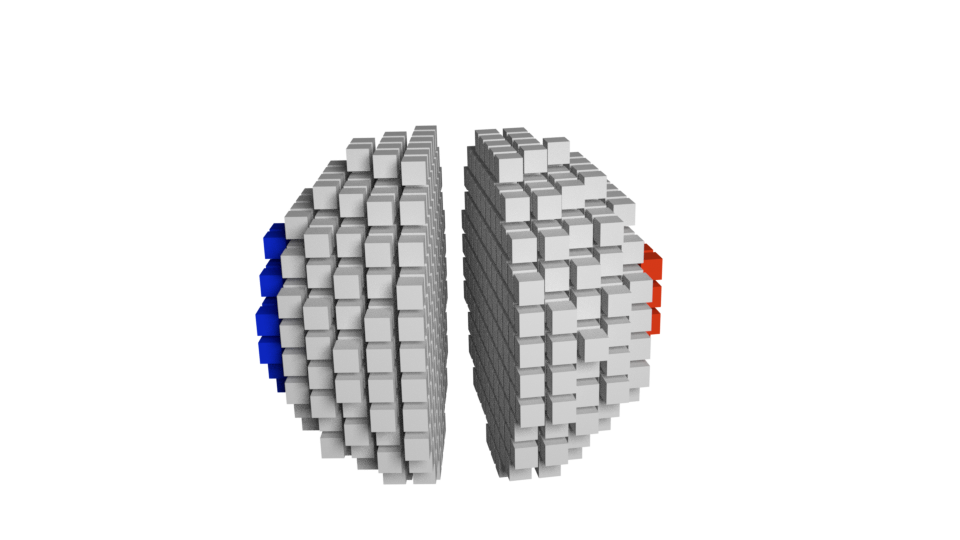
\includegraphics{media/pics/sliced_cube.png}
\caption{Numerical Grain}
\end{figure}

    \begin{tcolorbox}[breakable, size=fbox, boxrule=1pt, pad at break*=1mm,colback=cellbackground, colframe=cellborder]
\prompt{In}{incolor}{8}{\boxspacing}
\begin{Verbatim}[commandchars=\\\{\}]
\PY{k}{def} \PY{n+nf}{pos\PYZus{}to\PYZus{}r}\PY{p}{(}\PY{n}{xi}\PY{p}{,}\PY{n}{yi}\PY{p}{,}\PY{n}{grain}\PY{p}{,} \PY{n}{d}\PY{p}{)}\PY{p}{:}
    \PY{n}{dx} \PY{o}{=} \PY{l+m+mi}{2}\PY{o}{*}\PY{n}{grain}\PY{o}{.}\PY{n}{R}\PY{o}{/}\PY{n}{d}\PY{o}{.}\PY{n}{shape}\PY{p}{[}\PY{l+m+mi}{0}\PY{p}{]}
    \PY{n}{cx} \PY{o}{=} \PY{n}{d}\PY{o}{.}\PY{n}{shape}\PY{p}{[}\PY{l+m+mi}{0}\PY{p}{]}\PY{o}{/}\PY{o}{/}\PY{l+m+mi}{2}
    \PY{n}{cy} \PY{o}{=} \PY{n}{d}\PY{o}{.}\PY{n}{shape}\PY{p}{[}\PY{l+m+mi}{1}\PY{p}{]}\PY{o}{/}\PY{o}{/}\PY{l+m+mi}{2}
    \PY{n}{ri} \PY{o}{=} \PY{p}{(}\PY{p}{(}\PY{n}{xi}\PY{o}{\PYZhy{}}\PY{n}{cx}\PY{p}{)}\PY{o}{*}\PY{o}{*}\PY{l+m+mi}{2}\PY{o}{+}\PY{p}{(}\PY{n}{yi}\PY{o}{\PYZhy{}}\PY{n}{cy}\PY{p}{)}\PY{o}{*}\PY{o}{*}\PY{l+m+mi}{2}\PY{p}{)}\PY{o}{*}\PY{o}{*}\PY{l+m+mf}{0.5}
    \PY{k}{return}\PY{p}{(}\PY{n}{ri}\PY{o}{*}\PY{n}{dx}\PY{p}{)}


\PY{k}{def} \PY{n+nf}{create\PYZus{}numerical\PYZus{}grain\PYZus{}matrix}\PY{p}{(} \PY{n}{grain}\PY{p}{,} \PY{n}{ser}\PY{p}{,}\PY{n}{size\PYZus{}n}\PY{o}{=}\PY{l+m+mi}{100}\PY{p}{,}\PY{p}{)}\PY{p}{:}
    \PY{n}{n\PYZus{}int}\PY{p}{,} \PY{n}{v\PYZus{}int} \PY{o}{=} \PY{n}{get\PYZus{}interpolated\PYZus{}n\PYZus{}v}\PY{p}{(}\PY{n}{ser}\PY{p}{,} \PY{n}{grain}\PY{p}{)}
    \PY{n}{nx} \PY{o}{=} \PY{n}{ny} \PY{o}{=} \PY{n}{size\PYZus{}n}

    
    \PY{n}{d\PYZus{}v} \PY{o}{=} \PY{n}{np}\PY{o}{.}\PY{n}{zeros}\PY{p}{(}\PY{p}{(}\PY{l+m+mi}{2}\PY{o}{*}\PY{n}{nx}\PY{o}{+}\PY{l+m+mi}{1}\PY{p}{,}\PY{l+m+mi}{2}\PY{o}{*}\PY{n}{ny}\PY{o}{+}\PY{l+m+mi}{1}\PY{p}{)}\PY{p}{)}
    \PY{n}{d\PYZus{}cond} \PY{o}{=} \PY{n}{np}\PY{o}{.}\PY{n}{zeros}\PY{p}{(}\PY{p}{(}\PY{l+m+mi}{2}\PY{o}{*}\PY{n}{nx}\PY{o}{+}\PY{l+m+mi}{1}\PY{p}{,}\PY{l+m+mi}{2}\PY{o}{*}\PY{n}{ny}\PY{o}{+}\PY{l+m+mi}{1}\PY{p}{)}\PY{p}{)}
    \PY{n}{d\PYZus{}mask} \PY{o}{=} \PY{n}{np}\PY{o}{.}\PY{n}{zeros}\PY{p}{(}\PY{p}{(}\PY{l+m+mi}{2}\PY{o}{*}\PY{n}{nx}\PY{o}{+}\PY{l+m+mi}{1}\PY{p}{,}\PY{l+m+mi}{2}\PY{o}{*}\PY{n}{ny}\PY{o}{+}\PY{l+m+mi}{1}\PY{p}{)}\PY{p}{)}
    

    \PY{k}{for} \PY{n}{xi} \PY{o+ow}{in} \PY{n+nb}{range}\PY{p}{(}\PY{n}{d\PYZus{}cond}\PY{o}{.}\PY{n}{shape}\PY{p}{[}\PY{l+m+mi}{0}\PY{p}{]}\PY{p}{)}\PY{p}{:}
        \PY{k}{for} \PY{n}{yi} \PY{o+ow}{in} \PY{n+nb}{range}\PY{p}{(}\PY{n}{d\PYZus{}cond}\PY{o}{.}\PY{n}{shape}\PY{p}{[}\PY{l+m+mi}{1}\PY{p}{]}\PY{p}{)}\PY{p}{:}
            \PY{n}{r} \PY{o}{=} \PY{n+nb}{float}\PY{p}{(}\PY{n}{pos\PYZus{}to\PYZus{}r}\PY{p}{(}\PY{n}{xi}\PY{p}{,}\PY{n}{yi}\PY{p}{,}\PY{n}{grain}\PY{p}{,} \PY{n}{d\PYZus{}cond}\PY{p}{)}\PY{p}{)}
            \PY{k}{try}\PY{p}{:}
                \PY{n}{condu} \PY{o}{=} \PY{n}{n\PYZus{}int}\PY{p}{(}\PY{n}{r}\PY{p}{)}\PY{o}{/}\PY{n}{grain}\PY{o}{.}\PY{n}{material}\PY{o}{.}\PY{n}{nb}
                \PY{n}{d\PYZus{}cond}\PY{p}{[}\PY{n}{xi}\PY{p}{,} \PY{n}{yi}\PY{p}{]} \PY{o}{=} \PY{n}{condu}
                \PY{n}{d\PYZus{}mask}\PY{p}{[}\PY{n}{xi}\PY{p}{,}\PY{n}{yi}\PY{p}{]} \PY{o}{=} \PY{l+m+mi}{1}

            \PY{k}{except} \PY{n+ne}{ValueError}\PY{p}{:}
                \PY{c+c1}{\PYZsh{}outside the grain}
                \PY{n}{d\PYZus{}cond}\PY{p}{[}\PY{n}{xi}\PY{p}{,} \PY{n}{yi}\PY{p}{]} \PY{o}{=} \PY{l+m+mi}{0}
                \PY{n}{d\PYZus{}mask}\PY{p}{[}\PY{n}{xi}\PY{p}{,}\PY{n}{yi}\PY{p}{]} \PY{o}{=} \PY{l+m+mi}{0}
    \PY{k}{return} \PY{n}{d\PYZus{}v}\PY{p}{,} \PY{n}{d\PYZus{}cond}\PY{p}{,} \PY{n}{d\PYZus{}mask}
\end{Verbatim}
\end{tcolorbox}

    \hypertarget{precalc-the-numerical-grains-for-all-conditions}{%
\subsection{Precalc the numerical grains for all
conditions}\label{precalc-the-numerical-grains-for-all-conditions}}

    \begin{tcolorbox}[breakable, size=fbox, boxrule=1pt, pad at break*=1mm,colback=cellbackground, colframe=cellborder]
\prompt{In}{incolor}{119}{\boxspacing}
\begin{Verbatim}[commandchars=\\\{\}]
\PY{k}{for} \PY{n}{i}\PY{p}{,} \PY{n}{ser} \PY{o+ow}{in} \PY{n}{calc\PYZus{}dF}\PY{o}{.}\PY{n}{iterrows}\PY{p}{(}\PY{p}{)}\PY{p}{:}
    \PY{n+nb}{print}\PY{p}{(}\PY{l+s+sa}{f}\PY{l+s+s1}{\PYZsq{}}\PY{l+s+s1}{Initalized }\PY{l+s+s1}{\PYZob{}}\PY{l+s+s1}{i+1\PYZcb{} of }\PY{l+s+s1}{\PYZob{}}\PY{l+s+s1}{len(calc\PYZus{}dF)\PYZcb{}.}\PY{l+s+s1}{\PYZsq{}}\PY{p}{,} \PY{n}{end}\PY{o}{=}\PY{l+s+s1}{\PYZsq{}}\PY{l+s+se}{\PYZbs{}r}\PY{l+s+s1}{\PYZsq{}}\PY{p}{)}
    \PY{n}{grain} \PY{o}{=} \PY{n}{create\PYZus{}grain\PYZus{}from\PYZus{}data}\PY{p}{(}\PY{n}{ser}\PY{p}{)}
    \PY{n}{d\PYZus{}v}\PY{p}{,} \PY{n}{d\PYZus{}cond}\PY{p}{,}\PY{n}{d\PYZus{}mask} \PY{o}{=} \PY{n}{create\PYZus{}numerical\PYZus{}grain\PYZus{}matrix}\PY{p}{(} \PY{n}{grain}\PY{p}{,} \PY{n}{ser}\PY{p}{,}\PY{n}{size\PYZus{}n}\PY{o}{=}\PY{l+m+mi}{100}\PY{p}{)}
    \PY{n}{d\PYZus{}cond\PYZus{}plot} \PY{o}{=} \PY{n}{d\PYZus{}cond}\PY{o}{.}\PY{n}{copy}\PY{p}{(}\PY{p}{)}
    \PY{n}{d\PYZus{}cond\PYZus{}plot}\PY{p}{[}\PY{n}{np}\PY{o}{.}\PY{n}{where}\PY{p}{(}\PY{n}{d\PYZus{}mask}\PY{o}{==}\PY{l+m+mi}{0}\PY{p}{)}\PY{p}{]}\PY{o}{=}\PY{k+kc}{None}
    \PY{n}{calc\PYZus{}dF}\PY{o}{.}\PY{n}{loc}\PY{p}{[}\PY{n}{ser}\PY{o}{.}\PY{n}{name}\PY{p}{,} \PY{l+s+s1}{\PYZsq{}}\PY{l+s+s1}{d\PYZus{}cond}\PY{l+s+s1}{\PYZsq{}}\PY{p}{]} \PY{o}{=} \PY{p}{[}\PY{n}{d\PYZus{}cond\PYZus{}plot}\PY{p}{]}
\end{Verbatim}
\end{tcolorbox}

    \begin{Verbatim}[commandchars=\\\{\}]
Initalized 36 of 36.
    \end{Verbatim}

    \begin{tcolorbox}[breakable, size=fbox, boxrule=1pt, pad at break*=1mm,colback=cellbackground, colframe=cellborder]
\prompt{In}{incolor}{125}{\boxspacing}
\begin{Verbatim}[commandchars=\\\{\}]
\PY{o}{\PYZpc{}}\PY{k}{matplotlib} inline
\end{Verbatim}
\end{tcolorbox}

    This means in the accumulation layer there are a the specific position
5.39 times more free charge carriers available as in the center. This
results directly in a lower resistivity of the same factor. Instead of
just calculating just individual values, the graphical representation is
in this case more helpful.

    \begin{tcolorbox}[breakable, size=fbox, boxrule=1pt, pad at break*=1mm,colback=cellbackground, colframe=cellborder]
\prompt{In}{incolor}{126}{\boxspacing}
\begin{Verbatim}[commandchars=\\\{\}]
\PY{k}{def} \PY{n+nf}{plot\PYZus{}grain\PYZus{}states}\PY{p}{(}\PY{n}{calc\PYZus{}dF\PYZus{}grainsize}\PY{p}{,} \PY{n}{vmax}\PY{o}{=}\PY{k+kc}{None}\PY{p}{,} \PY{n}{vmin}\PY{o}{=}\PY{k+kc}{None}\PY{p}{)}\PY{p}{:}
    \PY{n}{fig}\PY{p}{,} \PY{n}{axes} \PY{o}{=} \PY{n}{subplots}\PY{p}{(}\PY{l+m+mi}{3}\PY{p}{,}\PY{l+m+mi}{3}\PY{p}{,} \PY{n}{figsize} \PY{o}{=} \PY{p}{(}\PY{l+m+mi}{16}\PY{p}{,}\PY{l+m+mi}{9}\PY{p}{)}\PY{p}{)}
    
    \PY{n}{grain} \PY{o}{=} \PY{n}{create\PYZus{}grain\PYZus{}from\PYZus{}data}\PY{p}{(}\PY{n}{calc\PYZus{}dF\PYZus{}grainsize}\PY{p}{)}

    \PY{k}{for} \PY{n}{ax\PYZus{}i}\PY{p}{,} \PY{p}{(}\PY{n}{vinit}\PY{p}{,} \PY{n}{ser}\PY{p}{)} \PY{o+ow}{in} \PY{n+nb}{enumerate}\PY{p}{(}\PY{n}{calc\PYZus{}dF\PYZus{}grainsize}\PY{o}{.}\PY{n}{iterrows}\PY{p}{(}\PY{p}{)}\PY{p}{)}\PY{p}{:}
        \PY{n}{axe} \PY{o}{=} \PY{n}{fig}\PY{o}{.}\PY{n}{axes}\PY{p}{[}\PY{n}{ax\PYZus{}i}\PY{p}{]}
        
        \PY{n}{Einit\PYZus{}kT} \PY{o}{=} \PY{n}{ser}\PY{p}{[}\PY{l+s+s1}{\PYZsq{}}\PY{l+s+s1}{Einit\PYZus{}kT}\PY{l+s+s1}{\PYZsq{}}\PY{p}{]}

        \PY{n}{axe}\PY{o}{.}\PY{n}{set\PYZus{}title}\PY{p}{(}\PY{l+s+sa}{r}\PY{l+s+s1}{\PYZsq{}}\PY{l+s+s1}{\PYZdl{}E\PYZus{}}\PY{l+s+s1}{\PYZob{}}\PY{l+s+s1}{C\PYZus{}}\PY{l+s+si}{\PYZob{}Surface\PYZcb{}}\PY{l+s+s1}{\PYZcb{}=\PYZdl{}}\PY{l+s+s1}{\PYZsq{}}\PY{o}{+}\PY{l+s+sa}{f}\PY{l+s+s1}{\PYZsq{}}\PY{l+s+si}{\PYZob{}Einit\PYZus{}kT\PYZcb{}}\PY{l+s+s1}{kT}\PY{l+s+s1}{\PYZsq{}}\PY{p}{)}
        \PY{n}{axe}\PY{o}{.}\PY{n}{set\PYZus{}ylabel}\PY{p}{(}\PY{l+s+s1}{\PYZsq{}}\PY{l+s+s1}{x [nm]}\PY{l+s+s1}{\PYZsq{}}\PY{p}{)}
        \PY{n}{axe}\PY{o}{.}\PY{n}{set\PYZus{}xlabel}\PY{p}{(}\PY{l+s+s1}{\PYZsq{}}\PY{l+s+s1}{y [nm]}\PY{l+s+s1}{\PYZsq{}}\PY{p}{)}
        
        \PY{n}{d\PYZus{}cond\PYZus{}plot} \PY{o}{=} \PY{n}{calc\PYZus{}dF}\PY{o}{.}\PY{n}{loc}\PY{p}{[}\PY{n}{ser}\PY{o}{.}\PY{n}{name}\PY{p}{,} \PY{l+s+s1}{\PYZsq{}}\PY{l+s+s1}{d\PYZus{}cond}\PY{l+s+s1}{\PYZsq{}}\PY{p}{]}
        \PY{n}{im} \PY{o}{=} \PY{n}{axe}\PY{o}{.}\PY{n}{imshow}\PY{p}{(}\PY{n}{np}\PY{o}{.}\PY{n}{log}\PY{p}{(}\PY{n}{d\PYZus{}cond\PYZus{}plot}\PY{p}{)}\PY{p}{,} \PY{n}{interpolation}\PY{o}{=}\PY{l+s+s1}{\PYZsq{}}\PY{l+s+s1}{bicubic}\PY{l+s+s1}{\PYZsq{}}\PY{p}{,}
                        \PY{n}{extent}\PY{o}{=}\PY{p}{(}\PY{o}{\PYZhy{}}\PY{n}{grain}\PY{o}{.}\PY{n}{R}\PY{o}{*}\PY{l+m+mf}{1e9}\PY{p}{,} \PY{n}{grain}\PY{o}{.}\PY{n}{R}\PY{o}{*}\PY{l+m+mf}{1e9}\PY{p}{,} \PY{o}{\PYZhy{}}\PY{n}{grain}\PY{o}{.}\PY{n}{R}\PY{o}{*}\PY{l+m+mf}{1e9}\PY{p}{,} \PY{n}{grain}\PY{o}{.}\PY{n}{R}\PY{o}{*}\PY{l+m+mf}{1e9}\PY{p}{)}\PY{p}{,}
                        \PY{n}{vmax}\PY{o}{=}\PY{n}{vmax}\PY{p}{,} \PY{n}{vmin}\PY{o}{=}\PY{n}{vmin}\PY{p}{,} \PY{n}{cmap}\PY{o}{=}\PY{l+s+s1}{\PYZsq{}}\PY{l+s+s1}{hot}\PY{l+s+s1}{\PYZsq{}}\PY{p}{)}
    \PY{n}{fig}\PY{o}{.}\PY{n}{tight\PYZus{}layout}\PY{p}{(}\PY{p}{)}
    


\PY{k}{def} \PY{n+nf}{plot\PYZus{}currents}\PY{p}{(}\PY{n}{GrainRadius}\PY{p}{)}\PY{p}{:}
    \PY{n}{R} \PY{o}{=} \PY{n}{GrainRadius}\PY{o}{/}\PY{l+m+mf}{1e9}
    \PY{n}{calc\PYZus{}dF\PYZus{}grainsize} \PY{o}{=} \PY{n}{calc\PYZus{}dF}\PY{o}{.}\PY{n}{groupby}\PY{p}{(}\PY{l+s+s1}{\PYZsq{}}\PY{l+s+s1}{R}\PY{l+s+s1}{\PYZsq{}}\PY{p}{)}\PY{o}{.}\PY{n}{get\PYZus{}group}\PY{p}{(}\PY{n}{R}\PY{p}{)}
    \PY{n}{max\PYZus{}n} \PY{o}{=} \PY{n}{np}\PY{o}{.}\PY{n}{log}\PY{p}{(}\PY{n}{calc\PYZus{}dF\PYZus{}grainsize}\PY{p}{[}\PY{l+s+s1}{\PYZsq{}}\PY{l+s+s1}{d\PYZus{}cond}\PY{l+s+s1}{\PYZsq{}}\PY{p}{]}\PY{o}{.}\PY{n}{apply}\PY{p}{(}\PY{k}{lambda} \PY{n}{r}\PY{p}{:}\PY{n}{np}\PY{o}{.}\PY{n}{nanmax}\PY{p}{(}\PY{n}{r}\PY{p}{)}\PY{p}{)}\PY{p}{)}\PY{o}{.}\PY{n}{max}\PY{p}{(}\PY{p}{)}
    \PY{n}{min\PYZus{}n} \PY{o}{=} \PY{n}{np}\PY{o}{.}\PY{n}{log}\PY{p}{(}\PY{n}{calc\PYZus{}dF\PYZus{}grainsize}\PY{p}{[}\PY{l+s+s1}{\PYZsq{}}\PY{l+s+s1}{d\PYZus{}cond}\PY{l+s+s1}{\PYZsq{}}\PY{p}{]}\PY{o}{.}\PY{n}{apply}\PY{p}{(}\PY{k}{lambda} \PY{n}{r}\PY{p}{:}\PY{n}{np}\PY{o}{.}\PY{n}{nanmin}\PY{p}{(}\PY{n}{r}\PY{p}{)}\PY{p}{)}\PY{p}{)}\PY{o}{.}\PY{n}{min}\PY{p}{(}\PY{p}{)}
    \PY{n+nb}{print}\PY{p}{(}\PY{n}{max\PYZus{}n}\PY{p}{,} \PY{n}{min\PYZus{}n}\PY{p}{)}
    
    \PY{n}{plot\PYZus{}grain\PYZus{}states}\PY{p}{(}\PY{n}{calc\PYZus{}dF\PYZus{}grainsize}\PY{p}{,} \PY{n}{vmax} \PY{o}{=} \PY{n}{max\PYZus{}n}\PY{p}{,} \PY{n}{vmin} \PY{o}{=} \PY{n}{min\PYZus{}n}\PY{p}{)}

\PY{n}{grainsizes} \PY{o}{=} \PY{n+nb}{list}\PY{p}{(}\PY{n}{calc\PYZus{}dF}\PY{p}{[}\PY{l+s+s1}{\PYZsq{}}\PY{l+s+s1}{R}\PY{l+s+s1}{\PYZsq{}}\PY{p}{]}\PY{o}{.}\PY{n}{unique}\PY{p}{(}\PY{p}{)}\PY{p}{)}
\PY{n}{interact}\PY{p}{(}\PY{n}{plot\PYZus{}currents}\PY{p}{,} \PY{n}{GrainRadius}\PY{o}{=}\PY{n}{np}\PY{o}{.}\PY{n}{array}\PY{p}{(}\PY{n}{grainsizes}\PY{p}{)}\PY{o}{*}\PY{l+m+mf}{1e9}\PY{p}{,} \PY{n}{text}\PY{o}{=}\PY{l+s+s1}{\PYZsq{}}\PY{l+s+s1}{Select a grainsize:}\PY{l+s+s1}{\PYZsq{}}\PY{p}{)}\PY{p}{;}
\end{Verbatim}
\end{tcolorbox}

    
    \begin{verbatim}
interactive(children=(Dropdown(description='GrainRadius', options=(50.0, 100.0, 200.0, 400.0), value=50.0), Ou…
    \end{verbatim}

    
    \hypertarget{relaxation}{%
\section{Relaxation}\label{relaxation}}

    \begin{tcolorbox}[breakable, size=fbox, boxrule=1pt, pad at break*=1mm,colback=cellbackground, colframe=cellborder]
\prompt{In}{incolor}{71}{\boxspacing}
\begin{Verbatim}[commandchars=\\\{\}]
\PY{n}{calc\PYZus{}dF}\PY{o}{.}\PY{n}{to\PYZus{}hdf}\PY{p}{(}\PY{l+s+s1}{\PYZsq{}}\PY{l+s+s1}{size\PYZus{}test\PYZus{}delete\PYZus{}please.h5}\PY{l+s+s1}{\PYZsq{}}\PY{p}{,} \PY{l+s+s1}{\PYZsq{}}\PY{l+s+s1}{raw}\PY{l+s+s1}{\PYZsq{}}\PY{p}{)}
\end{Verbatim}
\end{tcolorbox}

    \begin{Verbatim}[commandchars=\\\{\}]
/usr/lib/python3.8/site-packages/pandas/core/generic.py:2530:
PerformanceWarning:
your performance may suffer as PyTables will pickle object types that it cannot
map directly to c-types [inferred\_type->mixed,key->block1\_values] [items->['n',
'r', 'v', 'v\_dot', 'd\_cond']]

  pytables.to\_hdf(path\_or\_buf, key, self, **kwargs)
    \end{Verbatim}

    \begin{tcolorbox}[breakable, size=fbox, boxrule=1pt, pad at break*=1mm,colback=cellbackground, colframe=cellborder]
\prompt{In}{incolor}{68}{\boxspacing}
\begin{Verbatim}[commandchars=\\\{\}]
\PY{k+kn}{from} \PY{n+nn}{scipy} \PY{k+kn}{import} \PY{n}{signal}


\PY{k}{def} \PY{n+nf}{initaliz\PYZus{}d\PYZus{}v}\PY{p}{(}\PY{n}{d\PYZus{}v}\PY{p}{)}\PY{p}{:}
    \PY{n}{d\PYZus{}v}\PY{p}{[}\PY{p}{:}\PY{p}{,}\PY{l+m+mi}{0}\PY{p}{]} \PY{o}{=} \PY{o}{\PYZhy{}}\PY{l+m+mi}{1000}
    \PY{n}{d\PYZus{}v}\PY{p}{[}\PY{p}{:}\PY{p}{,}\PY{o}{\PYZhy{}}\PY{l+m+mi}{1}\PY{p}{]} \PY{o}{=} \PY{o}{+}\PY{l+m+mi}{1000}
    \PY{n}{d\PYZus{}v} \PY{o}{=} \PY{n}{d\PYZus{}v}\PY{o}{*}\PY{n}{d\PYZus{}mask}
    \PY{k}{return} \PY{n}{d\PYZus{}v}

\PY{k}{def} \PY{n+nf}{solve\PYZus{}relaxation}\PY{p}{(}\PY{n}{d\PYZus{}v}\PY{p}{,} \PY{n}{d\PYZus{}cond}\PY{p}{,} \PY{n}{d\PYZus{}mask}\PY{p}{)}\PY{p}{:}
    \PY{n}{res\PYZus{}new} \PY{o}{=} \PY{l+m+mi}{1000}
    \PY{k}{for} \PY{n}{i} \PY{o+ow}{in} \PY{n+nb}{range}\PY{p}{(}\PY{l+m+mi}{300000}\PY{p}{)}\PY{p}{:}

        \PY{n}{conv} \PY{o}{=} \PY{p}{[}\PY{p}{[}\PY{l+m+mi}{0}\PY{p}{,}\PY{l+m+mi}{1}\PY{p}{,}\PY{l+m+mi}{0}\PY{p}{]}\PY{p}{,}\PY{p}{[}\PY{l+m+mi}{1}\PY{p}{,}\PY{l+m+mi}{0}\PY{p}{,}\PY{l+m+mi}{1}\PY{p}{]}\PY{p}{,}\PY{p}{[}\PY{l+m+mi}{0}\PY{p}{,}\PY{l+m+mi}{1}\PY{p}{,}\PY{l+m+mi}{0}\PY{p}{]}\PY{p}{]}
        \PY{n}{numerator} \PY{o}{=} \PY{n}{signal}\PY{o}{.}\PY{n}{convolve2d}\PY{p}{(}\PY{n}{d\PYZus{}v}\PY{o}{*}\PY{n}{d\PYZus{}cond}\PY{p}{,} \PY{n}{conv}\PY{p}{,} \PY{n}{boundary}\PY{o}{=}\PY{l+s+s1}{\PYZsq{}}\PY{l+s+s1}{fill}\PY{l+s+s1}{\PYZsq{}}\PY{p}{,}
                                      \PY{n}{mode}\PY{o}{=}\PY{l+s+s1}{\PYZsq{}}\PY{l+s+s1}{same}\PY{l+s+s1}{\PYZsq{}}\PY{p}{,} \PY{n}{fillvalue}\PY{o}{=}\PY{l+m+mi}{0}\PY{p}{)}
        \PY{n}{denominator} \PY{o}{=} \PY{n}{signal}\PY{o}{.}\PY{n}{convolve2d}\PY{p}{(}\PY{n}{d\PYZus{}cond}\PY{p}{,} \PY{n}{conv}\PY{p}{,} \PY{n}{boundary}\PY{o}{=}\PY{l+s+s1}{\PYZsq{}}\PY{l+s+s1}{fill}\PY{l+s+s1}{\PYZsq{}}\PY{p}{,}
                                        \PY{n}{mode}\PY{o}{=}\PY{l+s+s1}{\PYZsq{}}\PY{l+s+s1}{same}\PY{l+s+s1}{\PYZsq{}}\PY{p}{,} \PY{n}{fillvalue}\PY{o}{=}\PY{l+m+mi}{0}\PY{p}{)}
        \PY{n}{d\PYZus{}v\PYZus{}new} \PY{o}{=} \PY{p}{(}\PY{n}{numerator}\PY{o}{/}\PY{n}{denominator}\PY{p}{)}\PY{o}{*}\PY{n}{d\PYZus{}mask}
        \PY{n}{d\PYZus{}v\PYZus{}new} \PY{o}{=} \PY{n}{np}\PY{o}{.}\PY{n}{nan\PYZus{}to\PYZus{}num}\PY{p}{(}\PY{n}{d\PYZus{}v\PYZus{}new}\PY{p}{,}\PY{l+m+mi}{0}\PY{p}{)}

        \PY{n}{d\PYZus{}v\PYZus{}prev} \PY{o}{=} \PY{n}{d\PYZus{}v}\PY{o}{.}\PY{n}{copy}\PY{p}{(}\PY{p}{)}
        

        
        \PY{n}{d\PYZus{}v} \PY{o}{=} \PY{n}{d\PYZus{}v\PYZus{}new}\PY{o}{.}\PY{n}{copy}\PY{p}{(}\PY{p}{)}
        \PY{n}{d\PYZus{}v} \PY{o}{=} \PY{n}{initaliz\PYZus{}d\PYZus{}v}\PY{p}{(}\PY{n}{d\PYZus{}v}\PY{p}{)}

        \PY{n}{res\PYZus{}pre} \PY{o}{=} \PY{n}{res\PYZus{}new}
        \PY{n}{res\PYZus{}new} \PY{o}{=} \PY{n}{np}\PY{o}{.}\PY{n}{abs}\PY{p}{(}\PY{n}{np}\PY{o}{.}\PY{n}{sum}\PY{p}{(}\PY{n}{d\PYZus{}v\PYZus{}prev}\PY{o}{\PYZhy{}}\PY{n}{d\PYZus{}v}\PY{p}{)}\PY{p}{)}

        \PY{k}{if} \PY{n}{i}\PY{o}{\PYZpc{}}\PY{k}{10000}==1:
            \PY{n+nb}{print}\PY{p}{(}\PY{n}{res\PYZus{}pre}\PY{p}{,}\PY{n}{res\PYZus{}new}\PY{p}{)}
            
            \PY{k}{if} \PY{p}{(}\PY{p}{(}\PY{n}{res\PYZus{}pre} \PY{o}{\PYZhy{}} \PY{n}{res\PYZus{}new}\PY{p}{)}\PY{o}{==}\PY{l+m+mi}{0}\PY{p}{)} \PY{o+ow}{and} \PY{p}{(}\PY{n}{i}\PY{o}{\PYZgt{}}\PY{l+m+mi}{40000}\PY{p}{)}\PY{p}{:}
                \PY{k}{break}
            
    \PY{k}{return} \PY{n}{d\PYZus{}v}\PY{p}{,} \PY{n}{d\PYZus{}cond}\PY{p}{,} \PY{n}{d\PYZus{}mask}

\PY{k}{def} \PY{n+nf}{plot\PYZus{}num\PYZus{}grain}\PY{p}{(}\PY{n}{d\PYZus{}v}\PY{p}{,} \PY{n}{d\PYZus{}cond}\PY{p}{,} \PY{n}{d\PYZus{}mask}\PY{p}{)}\PY{p}{:}
    \PY{n}{fig}\PY{p}{,} \PY{n}{axes} \PY{o}{=}\PY{n}{subplots}\PY{p}{(}\PY{l+m+mi}{1}\PY{p}{,}\PY{l+m+mi}{3}\PY{p}{)}
    \PY{n}{d\PYZus{}v\PYZus{}plot} \PY{o}{=} \PY{n}{d\PYZus{}v}\PY{o}{.}\PY{n}{copy}\PY{p}{(}\PY{p}{)}
    \PY{n}{d\PYZus{}v\PYZus{}plot}\PY{p}{[}\PY{n}{np}\PY{o}{.}\PY{n}{where}\PY{p}{(}\PY{n}{d\PYZus{}mask}\PY{o}{==}\PY{l+m+mi}{0}\PY{p}{)}\PY{p}{]}\PY{o}{=}\PY{k+kc}{None}

    \PY{n}{axes}\PY{p}{[}\PY{l+m+mi}{0}\PY{p}{]}\PY{o}{.}\PY{n}{imshow}\PY{p}{(}\PY{n}{d\PYZus{}mask}\PY{p}{)}
    \PY{n}{axes}\PY{p}{[}\PY{l+m+mi}{1}\PY{p}{]}\PY{o}{.}\PY{n}{imshow}\PY{p}{(}\PY{n}{d\PYZus{}cond}\PY{p}{)}
    \PY{n}{axes}\PY{p}{[}\PY{l+m+mi}{2}\PY{p}{]}\PY{o}{.}\PY{n}{imshow}\PY{p}{(}\PY{n}{d\PYZus{}v\PYZus{}plot}\PY{p}{,}\PY{n}{interpolation}\PY{o}{=} \PY{l+s+s1}{\PYZsq{}}\PY{l+s+s1}{nearest}\PY{l+s+s1}{\PYZsq{}}\PY{p}{)}
    
\PY{k}{def} \PY{n+nf}{plot\PYZus{}voltage\PYZus{}1d}\PY{p}{(}\PY{n}{d\PYZus{}v}\PY{p}{)}\PY{p}{:}
    \PY{n}{fig}\PY{p}{,} \PY{n}{axe} \PY{o}{=} \PY{n}{subplots}\PY{p}{(}\PY{p}{)}
    \PY{n}{center} \PY{o}{=} \PY{n}{d\PYZus{}v}\PY{p}{[}\PY{n}{d\PYZus{}v}\PY{o}{.}\PY{n}{shape}\PY{p}{[}\PY{l+m+mi}{0}\PY{p}{]}\PY{o}{/}\PY{o}{/}\PY{l+m+mi}{2}\PY{p}{,}\PY{p}{:}\PY{p}{]}
    \PY{n}{axe}\PY{o}{.}\PY{n}{plot}\PY{p}{(}\PY{n}{center}\PY{p}{)}

\PY{k}{def} \PY{n+nf}{calc\PYZus{}current\PYZus{}center}\PY{p}{(}\PY{n}{d\PYZus{}v}\PY{p}{,} \PY{n}{d\PYZus{}cond}\PY{p}{,} \PY{n}{d\PYZus{}mask}\PY{p}{)}\PY{p}{:}
    \PY{n}{center\PYZus{}pos} \PY{o}{=} \PY{n}{d\PYZus{}v}\PY{o}{.}\PY{n}{shape}\PY{p}{[}\PY{l+m+mi}{0}\PY{p}{]}\PY{o}{/}\PY{o}{/}\PY{l+m+mi}{2}
    \PY{n}{center\PYZus{}current} \PY{o}{=} \PY{p}{(}\PY{n}{d\PYZus{}v}\PY{p}{[}\PY{p}{:}\PY{p}{,}\PY{n}{center\PYZus{}pos}\PY{o}{+}\PY{l+m+mi}{1}\PY{p}{]}\PY{o}{\PYZhy{}}\PY{n}{d\PYZus{}v}\PY{p}{[}\PY{p}{:}\PY{p}{,}\PY{n}{center\PYZus{}pos}\PY{o}{\PYZhy{}}\PY{l+m+mi}{1}\PY{p}{]}\PY{p}{)}\PY{o}{*}\PY{n}{d\PYZus{}cond}\PY{p}{[}\PY{p}{:}\PY{p}{,}\PY{n}{center\PYZus{}pos}\PY{p}{]}
    
    \PY{n}{r} \PY{o}{=} \PY{n}{np}\PY{o}{.}\PY{n}{array}\PY{p}{(}\PY{p}{[}\PY{n+nb}{float}\PY{p}{(}\PY{n}{pos\PYZus{}to\PYZus{}r}\PY{p}{(}\PY{n}{xi}\PY{p}{,}\PY{n}{center\PYZus{}pos}\PY{p}{,}\PY{n}{grain}\PY{p}{,} \PY{n}{d\PYZus{}v}\PY{p}{)}\PY{p}{)} \PY{k}{for} \PY{n}{xi} \PY{o+ow}{in} \PY{n+nb}{range}\PY{p}{(}\PY{n+nb}{len}\PY{p}{(}\PY{n}{center\PYZus{}current}\PY{p}{)}\PY{p}{)}\PY{p}{]}\PY{p}{)}
    
    \PY{n}{center\PYZus{}current\PYZus{}tot} \PY{o}{=} \PY{n}{np}\PY{o}{.}\PY{n}{sum}\PY{p}{(}\PY{n}{center\PYZus{}current}\PY{o}{*}\PY{n}{r}\PY{o}{*}\PY{l+m+mi}{2}\PY{o}{*}\PY{n}{pi}\PY{p}{)}
    \PY{k}{return} \PY{n}{center\PYZus{}current\PYZus{}tot}\PY{p}{,} \PY{n}{center\PYZus{}current}\PY{p}{,} \PY{n}{r}

\PY{k}{def} \PY{n+nf}{plot\PYZus{}center\PYZus{}current}\PY{p}{(}\PY{n}{r}\PY{p}{,} \PY{n}{center\PYZus{}current}\PY{p}{)}\PY{p}{:}
    \PY{n}{fig}\PY{p}{,} \PY{n}{axe} \PY{o}{=} \PY{n}{subplots}\PY{p}{(}\PY{p}{)}
    \PY{n}{axe}\PY{o}{.}\PY{n}{plot}\PY{p}{(}\PY{n}{r}\PY{o}{*}\PY{l+m+mf}{1e9}\PY{p}{,}\PY{n}{center\PYZus{}current}\PY{p}{)}
    \PY{k}{return}

\PY{c+c1}{\PYZsh{}vinit, current = calc\PYZus{}current(d\PYZus{}v, d\PYZus{}cond, d\PYZus{}mask)}
\end{Verbatim}
\end{tcolorbox}

    \begin{tcolorbox}[breakable, size=fbox, boxrule=1pt, pad at break*=1mm,colback=cellbackground, colframe=cellborder]
\prompt{In}{incolor}{ }{\boxspacing}
\begin{Verbatim}[commandchars=\\\{\}]
\PY{n}{calc\PYZus{}dF}\PY{p}{[}\PY{l+s+s1}{\PYZsq{}}\PY{l+s+s1}{current}\PY{l+s+s1}{\PYZsq{}}\PY{p}{]} \PY{o}{=} \PY{k+kc}{None}
\end{Verbatim}
\end{tcolorbox}

    \begin{tcolorbox}[breakable, size=fbox, boxrule=1pt, pad at break*=1mm,colback=cellbackground, colframe=cellborder]
\prompt{In}{incolor}{ }{\boxspacing}
\begin{Verbatim}[commandchars=\\\{\}]
\PY{k}{def} \PY{n+nf}{initaliz\PYZus{}d\PYZus{}v}\PY{p}{(}\PY{n}{d\PYZus{}v}\PY{p}{)}\PY{p}{:}
    \PY{n}{d\PYZus{}v}\PY{p}{[}\PY{p}{:}\PY{p}{,}\PY{l+m+mi}{0}\PY{p}{]} \PY{o}{=} \PY{o}{\PYZhy{}}\PY{l+m+mi}{1000}
    \PY{n}{d\PYZus{}v}\PY{p}{[}\PY{p}{:}\PY{p}{,}\PY{o}{\PYZhy{}}\PY{l+m+mi}{1}\PY{p}{]} \PY{o}{=} \PY{o}{+}\PY{l+m+mi}{1000}
    \PY{n}{d\PYZus{}v} \PY{o}{=} \PY{n}{d\PYZus{}v}\PY{o}{*}\PY{n}{d\PYZus{}mask}
    \PY{k}{return} \PY{n}{d\PYZus{}v}


\PY{c+c1}{\PYZsh{}for vinit, ser in calc\PYZus{}dF.iterrows():}
\PY{n}{calc\PYZus{}dFs} \PY{o}{=} \PY{p}{\PYZob{}}\PY{p}{\PYZcb{}}
\PY{k}{for} \PY{n}{size\PYZus{}n} \PY{o+ow}{in} \PY{p}{[}\PY{l+m+mi}{10}\PY{p}{,}\PY{l+m+mi}{20}\PY{p}{,}\PY{l+m+mi}{40}\PY{p}{]}\PY{p}{:}
    \PY{n}{c\PYZus{}dF} \PY{o}{=} \PY{n}{calc\PYZus{}dF}\PY{o}{.}\PY{n}{copy}\PY{p}{(}\PY{p}{)}
    \PY{k}{for} \PY{n}{i}\PY{p}{,} \PY{p}{(}\PY{n}{ind}\PY{p}{,}\PY{n}{ser}\PY{p}{)} \PY{o+ow}{in} \PY{n+nb}{enumerate}\PY{p}{(}\PY{n}{c\PYZus{}dF}\PY{o}{.}\PY{n}{iterrows}\PY{p}{(}\PY{p}{)}\PY{p}{)}\PY{p}{:}

        \PY{n+nb}{print}\PY{p}{(}\PY{l+s+sa}{f}\PY{l+s+s1}{\PYZsq{}}\PY{l+s+s1}{Initalized }\PY{l+s+s1}{\PYZob{}}\PY{l+s+s1}{i+1\PYZcb{} of }\PY{l+s+s1}{\PYZob{}}\PY{l+s+s1}{len(c\PYZus{}dF)\PYZcb{}.}\PY{l+s+s1}{\PYZsq{}}\PY{p}{)}
        \PY{n}{vinit} \PY{o}{=} \PY{n}{ser}\PY{o}{.}\PY{n}{name}

        \PY{n}{grain} \PY{o}{=} \PY{n}{create\PYZus{}grain\PYZus{}from\PYZus{}data}\PY{p}{(}\PY{n}{ser}\PY{p}{)}

        \PY{n}{d\PYZus{}v}\PY{p}{,} \PY{n}{d\PYZus{}cond}\PY{p}{,} \PY{n}{d\PYZus{}mask} \PY{o}{=} \PY{n}{create\PYZus{}numerical\PYZus{}grain\PYZus{}matrix}\PY{p}{(} \PY{n}{grain}\PY{p}{,} \PY{n}{ser}\PY{p}{,}\PY{n}{size\PYZus{}n}\PY{o}{=}\PY{l+m+mi}{50}\PY{p}{,}\PY{p}{)}
        \PY{n}{d\PYZus{}v} \PY{o}{=} \PY{n}{initaliz\PYZus{}d\PYZus{}v}\PY{p}{(}\PY{n}{d\PYZus{}v}\PY{p}{)}

        \PY{n}{d\PYZus{}v}\PY{p}{,} \PY{n}{d\PYZus{}cond}\PY{p}{,} \PY{n}{d\PYZus{}mask} \PY{o}{=} \PY{n}{solve\PYZus{}relaxation}\PY{p}{(}\PY{n}{d\PYZus{}v}\PY{p}{,} \PY{n}{d\PYZus{}cond}\PY{p}{,} \PY{n}{d\PYZus{}mask}\PY{p}{)}

        \PY{n}{center\PYZus{}current\PYZus{}tot}\PY{p}{,} \PY{n}{center\PYZus{}current}\PY{p}{,} \PY{n}{r} \PY{o}{=} \PY{n}{calc\PYZus{}current\PYZus{}center}\PY{p}{(}\PY{n}{d\PYZus{}v}\PY{p}{,} \PY{n}{d\PYZus{}cond}\PY{p}{,} \PY{n}{d\PYZus{}mask}\PY{p}{)}

        \PY{c+c1}{\PYZsh{}plot\PYZus{}num\PYZus{}grain(d\PYZus{}v, d\PYZus{}cond, d\PYZus{}mask)}
        \PY{c+c1}{\PYZsh{}plot\PYZus{}voltage\PYZus{}1d(d\PYZus{}v)}
        \PY{c+c1}{\PYZsh{}plot\PYZus{}center\PYZus{}current(r, center\PYZus{}current)}


        \PY{n}{c\PYZus{}dF}\PY{o}{.}\PY{n}{loc}\PY{p}{[}\PY{n}{vinit}\PY{p}{,} \PY{l+s+s1}{\PYZsq{}}\PY{l+s+s1}{current}\PY{l+s+s1}{\PYZsq{}}\PY{p}{]} \PY{o}{=} \PY{n}{center\PYZus{}current\PYZus{}tot}
    \PY{n}{calc\PYZus{}dFs}\PY{p}{[}\PY{n}{size\PYZus{}n}\PY{p}{]} \PY{o}{=} \PY{n}{c\PYZus{}dF}
\end{Verbatim}
\end{tcolorbox}

    \begin{Verbatim}[commandchars=\\\{\}]
Initalized 1 of 36.
2.8421709430404007e-13 3.979039320256561e-13
    \end{Verbatim}

    \begin{Verbatim}[commandchars=\\\{\}]
<ipython-input-68-1b3f12e4d0a4>:19: RuntimeWarning: invalid value encountered in
true\_divide
  d\_v\_new = (numerator/denominator)*d\_mask
    \end{Verbatim}

    \begin{Verbatim}[commandchars=\\\{\}]
5.597540660151612e-12 4.576233489372861e-12
1.534220671242214e-11 1.3914914007281606e-12
4.470048746920325e-12 9.824756458610649e-13
1.2982962227449369e-12 4.9067444464892115e-12
6.310799948503871e-12 8.070782245840193e-12
5.259566807207092e-13 5.955744226087447e-12
1.9950305793247724e-15 1.9950305793247724e-15
Initalized 2 of 36.
5.684341886080802e-14 2.5579538487363607e-13
2.7046333922475796e-13 2.5238413789430147e-12
6.63237348003695e-12 4.1252248538241505e-12
1.516062844756055e-12 2.4874125565111813e-12
7.101240957025582e-12 1.0338585944288182e-11
4.50583091424989e-13 3.977558506897941e-12
7.02315082651593e-13 7.02315082651593e-13
Initalized 3 of 36.
5.684341886080802e-14 1.9895196601282805e-13
5.085846674357519e-12 6.41049409735861e-12
3.456375115995112e-13 3.5217435250586154e-12
1.6061205840230561e-12 5.265787746054825e-12
2.5473353840283703e-13 3.720782808063357e-12
2.378961624638754e-12 1.986330415174384e-13
1.362542829301528e-15 1.362542829301528e-15
Initalized 4 of 36.
2.842170943040401e-14 2.842170943040401e-14
2.8745842511890274e-12 2.4342351051531708e-12
1.6601521242451205e-12 6.545235714365289e-13
7.312287233320852e-14 1.3091852729396762e-12
7.208215552573184e-12 5.875208580770587e-12
3.1035781812945857e-12 3.2519876812334817e-12
1.0799524540605742e-13 1.0799524540605742e-13
Initalized 5 of 36.
0.0 0.0
5.988775014093006e-13 4.9788732164879335e-14
1.1080208058778982e-12 1.2440246468186202e-12
8.428006193504832e-13 2.291528127233719e-12
3.1497713659841334e-12 2.2479316475194617e-12
1.0541576092378623e-12 4.2184183816408204e-13
2.0534699425693611e-13 2.0534699425693611e-13
Initalized 6 of 36.
0.0 0.0
4.217877999992958e-12 5.151807799808061e-13
9.447992916654705e-13 2.0567972086100615e-12
5.07786560688799e-14 1.1710913485430433e-12
8.280387703390536e-13 1.9880839601648235e-12
3.294696847146647e-14 3.294696847146647e-14
Initalized 7 of 36.
0.0 5.684341886080802e-14
4.258607138804549e-12 7.924336100501028e-13
3.0950570424848273e-13 6.751116445038525e-12
2.430741788159291e-12 6.527997379711602e-13
4.456502642525682e-12 1.5631201875501616e-12
7.100857292633375e-13 7.100857292633375e-13
Initalized 8 of 36.
0.0 8.526512829121202e-14
3.1715461420306346e-12 2.1528737993714575e-12
5.630016237927356e-13 1.488177698934001e-12
5.156239532828461e-12 1.4965758861951817e-12
2.2316575600712766e-12 5.298499217240854e-13
6.972631956475532e-13 6.972631956475532e-13
Initalized 9 of 36.
1.4210854715202004e-13 5.684341886080802e-14
2.444986921257275e-12 3.6159762250437266e-12
1.6330706945289148e-12 6.839813076170269e-13
1.1804550507101527e-12 2.7088343410589954e-12
2.901675828175278e-12 2.797562075880844e-12
1.2616599996386215e-12 1.2616599996386215e-12
Initalized 10 of 36.
1.1368683772161603e-13 5.684341886080802e-14
3.3999192350364638e-12 4.966981687060112e-13
5.181323631860829e-12 3.915407196597789e-12
7.988558698874144e-12 4.5378277581239405e-13
3.702032851986448e-12 4.280819884377772e-12
1.8835056746955e-12 7.620001335288423e-13
5.319452598921925e-12 3.2553786553245324e-13
1.0172979385391393e-12 1.0172979385391393e-12
Initalized 11 of 36.
5.684341886080802e-14 2.2737367544323206e-13
1.4724450825287505e-11 5.73276842663617e-12
6.821459751769378e-12 3.8352692400514705e-12
4.198526618973189e-12 2.1690548855709695e-12
7.331937156099569e-12 3.3154180239268447e-12
4.843110883206151e-12 4.225079059899676e-12
1.737693643603272e-13 1.737693643603272e-13
Initalized 12 of 36.
0.0 1.7053025658242404e-13
6.468937364945138e-12 2.4051489966314676e-12
6.51472046644399e-12 4.673052682389444e-13
1.888434082395351e-12 1.007659592609514e-12
7.482643522170005e-12 2.6847713676930836e-13
3.837900540431513e-12 4.7483793181592176e-12
7.348582024205915e-14 7.348582024205915e-14
Initalized 13 of 36.
5.684341886080802e-14 1.1368683772161603e-13
4.174467195527942e-12 4.1668968622787794e-13
1.0023013997684802e-12 1.1984212789349115e-12
5.2888142532237046e-12 3.299331160890803e-12
5.260471830203528e-12 6.6224766295278796e-12
6.758095012170122e-12 5.549388789789065e-12
1.0615337802961253e-13 1.0615337802961253e-13
Initalized 14 of 36.
0.0 0.0
5.988775014093006e-13 4.9788732164879335e-14
1.1080208058778982e-12 1.2440246468186202e-12
8.428006193504832e-13 2.291528127233719e-12
3.1497713659841334e-12 2.2479316475194617e-12
1.0541576092378623e-12 4.2184183816408204e-13
2.0534699425693611e-13 2.0534699425693611e-13
Initalized 15 of 36.
0.0 1.1368683772161603e-13
2.7712644462205005e-12 1.5357498259205293e-12
1.0609707417191794e-13 1.819116341597398e-12
1.333772164133691e-12 5.831894587454871e-13
3.0273595121384197e-13 6.274159430819693e-13
5.841400980135016e-14 5.841400980135016e-14
Initalized 16 of 36.
2.842170943040401e-14 1.1368683772161603e-13
2.519174105430899e-13 5.0387059975787185e-12
1.5287762909101782e-12 1.1115385698126247e-12
2.654297937887859e-14 3.6620468893999187e-13
2.979832425792127e-12 7.6184141596583e-13
2.1956875174490835e-13 2.1956875174490835e-13
Initalized 17 of 36.
1.1368683772161603e-13 1.9895196601282805e-13
1.5126246609431515e-12 7.943991601686018e-13
4.213449261811399e-13 2.1171197332983393e-12
1.2416092188741407e-12 2.0302840366419047e-13
2.590899154442774e-12 2.381036813953793e-13
4.341206153941698e-13 4.341206153941698e-13
Initalized 18 of 36.
2.842170943040401e-14 5.684341886080802e-14
1.7067390252825665e-12 1.625404184076723e-12
1.650857711230117e-12 4.4644500279367586e-12
2.623964729442451e-13 1.7853956947154557e-13
2.3948921357840345e-12 2.142541963385332e-12
4.539983958089127e-14 4.539983958089127e-14
Initalized 19 of 36.
2.2737367544323206e-13 5.684341886080802e-14
2.675349525249615e-12 6.1085095315327465e-12
7.165056525523794e-12 7.10954168800515e-12
5.171357157600365e-12 8.645265899649354e-13
9.784070593335905e-12 2.129667260912925e-11
9.752880823009038e-13 9.061693481960797e-12
1.4170204631795178e-13 2.6989768430341797e-12
6.869652001457677e-12 1.0236451190320722e-11
7.922364324115832e-12 1.670877441277303e-13
2.9843336315102916e-12 3.901005819203936e-12
5.390999848853081e-13 5.390999848853081e-13
Initalized 20 of 36.
5.684341886080802e-14 1.1368683772161603e-13
9.291840734337864e-12 3.5706030146465118e-12
2.3919873175823163e-12 3.989411780796776e-12
4.120949783777547e-12 1.2099002512460692e-11
1.7255894430786844e-12 1.2270909942196743e-12
2.297922441500996e-12 7.241104677425999e-12
8.938387826179157e-14 8.938387826179157e-14
Initalized 21 of 36.
5.684341886080802e-14 1.7053025658242404e-13
5.4586101264075815e-12 5.466000915776981e-12
8.194865803063138e-12 8.785424373668888e-12
1.3821806522857226e-13 5.4892736178927884e-12
2.77114332874572e-12 1.466248932295159e-12
4.091038979375689e-12 3.3010714795255397e-13
1.8510570506440295e-15 1.8510570506440295e-15
Initalized 22 of 36.
5.684341886080802e-14 2.842170943040401e-14
2.487911352627714e-12 1.335328549123549e-12
6.695592929243819e-12 3.5960784707417563e-12
8.762750628379257e-12 9.954437656593479e-13
3.822953546132045e-12 4.1443327323694594e-12
3.338448307306082e-13 4.802069866126378e-12
4.708930217608658e-13 4.708930217608658e-13
Initalized 23 of 36.
0.0 0.0
5.988775014093006e-13 4.9788732164879335e-14
1.1080208058778982e-12 1.2440246468186202e-12
8.428006193504832e-13 2.291528127233719e-12
3.1497713659841334e-12 2.2479316475194617e-12
1.0541576092378623e-12 4.2184183816408204e-13
2.0534699425693611e-13 2.0534699425693611e-13
Initalized 24 of 36.
2.842170943040401e-14 0.0
3.6647692259333953e-13 2.1521229893670113e-12
3.1345153728952127e-12 2.285115797798592e-12
1.3965368505233717e-12 1.1857748715938279e-12
1.8073021457620938e-12 2.4436201146981474e-12
1.6908523656192116e-14 1.6908523656192116e-14
Initalized 25 of 36.
2.842170943040401e-14 0.0
8.223672123049836e-13 1.0428012077977333e-12
2.981706114299935e-13 6.542987354808483e-13
2.5133274632064356e-13 3.1542613445079435e-13
1.4919408579082716e-12 6.554686723132359e-13
9.427523184383768e-14 9.427523184383768e-14
Initalized 26 of 36.
2.842170943040401e-14 2.842170943040401e-14
3.9526791070135695e-13 1.9589397590291505e-13
4.981187829964059e-13 4.95564873136051e-13
5.8098567786196195e-15 5.8098567786196195e-15
5.8098567786196195e-15 5.8098567786196195e-15
Initalized 27 of 36.
2.842170943040401e-14 2.842170943040401e-14
5.6923444984924e-13 1.2201235596677884e-13
1.1580276788707425e-16 1.1580276788707425e-16
1.1580276788707425e-16 1.1580276788707425e-16
1.1580276788707425e-16 1.1580276788707425e-16
Initalized 28 of 36.
3.410605131648481e-13 2.8421709430404007e-13
4.276426435190217e-12 1.9515777882617158e-12
2.9661030576111358e-12 6.707058519683784e-12
2.6938043809487944e-12 9.901361197953151e-12
3.882727527080437e-12 3.378156207458488e-12
5.837584145999657e-12 7.134998294229186e-13
1.9196979465454676e-12 1.5741431646539147e-12
1.6968939935238818e-13 2.1110071308870883e-13
8.823539733976676e-12 1.545019059420044e-11
5.432732220765718e-12 6.881437571794029e-12
6.471575826405922e-12 3.471213245019206e-12
9.369985699038109e-12 1.2311294078688313e-11
8.26312620751029e-12 1.2608653942040263e-11
1.7597940965352625e-11 2.302268833780088e-11
1.9897305468422964e-11 7.4718998875868e-12
1.7500368289384223e-11 1.1486881327393065e-11
3.9241534155638196e-12 2.191847952082073e-12
1.3545318650852653e-11 2.3388841923135747e-11
6.762014153042444e-13 6.762014153042444e-13
Initalized 29 of 36.
0.0 5.684341886080802e-14
3.180611156394786e-12 7.80502745767464e-12
1.636089633455344e-12 4.175821675749501e-12
2.6912740256611762e-12 1.8216408304407025e-12
2.4490971319719274e-12 2.8488891362605513e-12
1.3220632868992173e-12 4.5475244246014425e-12
1.4352554353356289e-12 5.728559133215052e-12
5.863976078308973e-13 5.863976078308973e-13
Initalized 30 of 36.
0.0 1.1368683772161603e-13
2.2908541383315217e-12 3.876778238709466e-12
2.7087241175375535e-12 5.356489435489296e-12
4.8941896219025894e-12 1.4779233915688463e-12
3.1106763474780303e-12 6.477422111857448e-13
1.469568805563763e-11 8.63064001145556e-12
4.483100812879532e-14 4.483100812879532e-14
Initalized 31 of 36.
0.0 2.842170943040401e-14
2.209153433102573e-12 3.962077627789329e-12
3.703776217167177e-12 1.2833142158669023e-13
2.362552905570715e-12 3.0091313754003794e-12
1.6988234046999665e-12 7.145900852554702e-13
1.4909204933266644e-12 1.0728146900197236e-12
2.344796931033319e-13 2.344796931033319e-13
Initalized 32 of 36.
0.0 0.0
5.988775014093006e-13 4.9788732164879335e-14
1.1080208058778982e-12 1.2440246468186202e-12
8.428006193504832e-13 2.291528127233719e-12
3.1497713659841334e-12 2.2479316475194617e-12
1.0541576092378623e-12 4.2184183816408204e-13
2.0534699425693611e-13 2.0534699425693611e-13
Initalized 33 of 36.
2.842170943040401e-14 2.842170943040401e-14
1.3471862514435884e-12 1.1774539676601137e-12
1.0602707769849745e-12 1.7368670097403808e-12
3.0910870673994e-12 3.162295432666544e-13
4.549784706837082e-13 2.569787389148047e-12
9.265653644767455e-13 6.4180320064244e-14
3.336881772012884e-13 3.336881772012884e-13
Initalized 34 of 36.
0.0 5.684341886080802e-14
1.1715195870690143e-12 9.820930960829921e-14
4.588008670778563e-13 7.068461933457571e-13
1.7381891084424414e-12 6.759791765697441e-13
3.504736454576228e-14 1.760579258131913e-12
2.7678573141506063e-13 3.270246293457977e-14
3.790482245862755e-15 3.790482245862755e-15
Initalized 35 of 36.
0.0 7.105427357601002e-14
2.2720449755267696e-13 2.2820547365589704e-14
4.094244386208744e-14 3.059031135325459e-14
1.2750546917967644e-13 3.727411996097038e-13
2.332783987798677e-13 7.498693655578753e-14
1.1375811565110507e-14 1.1375811565110507e-14
Initalized 36 of 36.
2.842170943040401e-14 2.842170943040401e-14
1.2559904932018158e-13 8.137811772874752e-14
2.0019242520961085e-14 1.8252382402752627e-14
7.356356642732609e-18 7.356356642732609e-18
7.356356642732609e-18 7.356356642732609e-18
Initalized 1 of 36.
2.8421709430404007e-13 3.979039320256561e-13
5.597540660151612e-12 4.576233489372861e-12
1.534220671242214e-11 1.3914914007281606e-12
4.470048746920325e-12 9.824756458610649e-13
1.2982962227449369e-12 4.9067444464892115e-12
6.310799948503871e-12 8.070782245840193e-12
5.259566807207092e-13 5.955744226087447e-12
1.9950305793247724e-15 1.9950305793247724e-15
Initalized 2 of 36.
5.684341886080802e-14 2.5579538487363607e-13
2.7046333922475796e-13 2.5238413789430147e-12
6.63237348003695e-12 4.1252248538241505e-12
1.516062844756055e-12 2.4874125565111813e-12
7.101240957025582e-12 1.0338585944288182e-11
4.50583091424989e-13 3.977558506897941e-12
7.02315082651593e-13 7.02315082651593e-13
Initalized 3 of 36.
5.684341886080802e-14 1.9895196601282805e-13
5.085846674357519e-12 6.41049409735861e-12
3.456375115995112e-13 3.5217435250586154e-12
1.6061205840230561e-12 5.265787746054825e-12
2.5473353840283703e-13 3.720782808063357e-12
2.378961624638754e-12 1.986330415174384e-13
1.362542829301528e-15 1.362542829301528e-15
Initalized 4 of 36.
2.842170943040401e-14 2.842170943040401e-14
2.8745842511890274e-12 2.4342351051531708e-12
1.6601521242451205e-12 6.545235714365289e-13
7.312287233320852e-14 1.3091852729396762e-12
7.208215552573184e-12 5.875208580770587e-12
3.1035781812945857e-12 3.2519876812334817e-12
1.0799524540605742e-13 1.0799524540605742e-13
Initalized 5 of 36.
0.0 0.0
5.988775014093006e-13 4.9788732164879335e-14
1.1080208058778982e-12 1.2440246468186202e-12
8.428006193504832e-13 2.291528127233719e-12
3.1497713659841334e-12 2.2479316475194617e-12
1.0541576092378623e-12 4.2184183816408204e-13
2.0534699425693611e-13 2.0534699425693611e-13
Initalized 6 of 36.
0.0 0.0
4.217877999992958e-12 5.151807799808061e-13
9.447992916654705e-13 2.0567972086100615e-12
5.07786560688799e-14 1.1710913485430433e-12
8.280387703390536e-13 1.9880839601648235e-12
3.294696847146647e-14 3.294696847146647e-14
Initalized 7 of 36.
0.0 5.684341886080802e-14
4.258607138804549e-12 7.924336100501028e-13
3.0950570424848273e-13 6.751116445038525e-12
2.430741788159291e-12 6.527997379711602e-13
4.456502642525682e-12 1.5631201875501616e-12
7.100857292633375e-13 7.100857292633375e-13
Initalized 8 of 36.
0.0 8.526512829121202e-14
3.1715461420306346e-12 2.1528737993714575e-12
5.630016237927356e-13 1.488177698934001e-12
5.156239532828461e-12 1.4965758861951817e-12
2.2316575600712766e-12 5.298499217240854e-13
6.972631956475532e-13 6.972631956475532e-13
Initalized 9 of 36.
1.4210854715202004e-13 5.684341886080802e-14
2.444986921257275e-12 3.6159762250437266e-12
1.6330706945289148e-12 6.839813076170269e-13
1.1804550507101527e-12 2.7088343410589954e-12
2.901675828175278e-12 2.797562075880844e-12
1.2616599996386215e-12 1.2616599996386215e-12
Initalized 10 of 36.
1.1368683772161603e-13 5.684341886080802e-14
3.3999192350364638e-12 4.966981687060112e-13
5.181323631860829e-12 3.915407196597789e-12
7.988558698874144e-12 4.5378277581239405e-13
3.702032851986448e-12 4.280819884377772e-12
1.8835056746955e-12 7.620001335288423e-13
5.319452598921925e-12 3.2553786553245324e-13
1.0172979385391393e-12 1.0172979385391393e-12
Initalized 11 of 36.
5.684341886080802e-14 2.2737367544323206e-13
1.4724450825287505e-11 5.73276842663617e-12
6.821459751769378e-12 3.8352692400514705e-12
4.198526618973189e-12 2.1690548855709695e-12
7.331937156099569e-12 3.3154180239268447e-12
4.843110883206151e-12 4.225079059899676e-12
1.737693643603272e-13 1.737693643603272e-13
Initalized 12 of 36.
0.0 1.7053025658242404e-13
6.468937364945138e-12 2.4051489966314676e-12
6.51472046644399e-12 4.673052682389444e-13
1.888434082395351e-12 1.007659592609514e-12
7.482643522170005e-12 2.6847713676930836e-13
3.837900540431513e-12 4.7483793181592176e-12
7.348582024205915e-14 7.348582024205915e-14
Initalized 13 of 36.
5.684341886080802e-14 1.1368683772161603e-13
4.174467195527942e-12 4.1668968622787794e-13
1.0023013997684802e-12 1.1984212789349115e-12
5.2888142532237046e-12 3.299331160890803e-12
5.260471830203528e-12 6.6224766295278796e-12
6.758095012170122e-12 5.549388789789065e-12
1.0615337802961253e-13 1.0615337802961253e-13
Initalized 14 of 36.
0.0 0.0
5.988775014093006e-13 4.9788732164879335e-14
1.1080208058778982e-12 1.2440246468186202e-12
8.428006193504832e-13 2.291528127233719e-12
3.1497713659841334e-12 2.2479316475194617e-12
1.0541576092378623e-12 4.2184183816408204e-13
2.0534699425693611e-13 2.0534699425693611e-13
Initalized 15 of 36.
0.0 1.1368683772161603e-13
2.7712644462205005e-12 1.5357498259205293e-12
1.0609707417191794e-13 1.819116341597398e-12
1.333772164133691e-12 5.831894587454871e-13
3.0273595121384197e-13 6.274159430819693e-13
5.841400980135016e-14 5.841400980135016e-14
Initalized 16 of 36.
2.842170943040401e-14 1.1368683772161603e-13
2.519174105430899e-13 5.0387059975787185e-12
1.5287762909101782e-12 1.1115385698126247e-12
2.654297937887859e-14 3.6620468893999187e-13
2.979832425792127e-12 7.6184141596583e-13
2.1956875174490835e-13 2.1956875174490835e-13
Initalized 17 of 36.
1.1368683772161603e-13 1.9895196601282805e-13
1.5126246609431515e-12 7.943991601686018e-13
4.213449261811399e-13 2.1171197332983393e-12
    \end{Verbatim}

    \begin{tcolorbox}[breakable, size=fbox, boxrule=1pt, pad at break*=1mm,colback=cellbackground, colframe=cellborder]
\prompt{In}{incolor}{52}{\boxspacing}
\begin{Verbatim}[commandchars=\\\{\}]
\PY{l+m+mf}{1e\PYZhy{}50}
\end{Verbatim}
\end{tcolorbox}

            \begin{tcolorbox}[breakable, size=fbox, boxrule=.5pt, pad at break*=1mm, opacityfill=0]
\prompt{Out}{outcolor}{52}{\boxspacing}
\begin{Verbatim}[commandchars=\\\{\}]
1e-50
\end{Verbatim}
\end{tcolorbox}
        
    \begin{tcolorbox}[breakable, size=fbox, boxrule=1pt, pad at break*=1mm,colback=cellbackground, colframe=cellborder]
\prompt{In}{incolor}{86}{\boxspacing}
\begin{Verbatim}[commandchars=\\\{\}]
\PY{n+nb}{len}\PY{p}{(}\PY{n}{calc\PYZus{}dFs}\PY{p}{[}\PY{l+m+mi}{10}\PY{p}{]}\PY{p}{)}
\end{Verbatim}
\end{tcolorbox}

            \begin{tcolorbox}[breakable, size=fbox, boxrule=.5pt, pad at break*=1mm, opacityfill=0]
\prompt{Out}{outcolor}{86}{\boxspacing}
\begin{Verbatim}[commandchars=\\\{\}]
36
\end{Verbatim}
\end{tcolorbox}
        
    \begin{tcolorbox}[breakable, size=fbox, boxrule=1pt, pad at break*=1mm,colback=cellbackground, colframe=cellborder]
\prompt{In}{incolor}{77}{\boxspacing}
\begin{Verbatim}[commandchars=\\\{\}]
\PY{n}{currents} \PY{o}{=} \PY{p}{[}\PY{p}{]}
\PY{n}{sizes} \PY{o}{=} \PY{p}{[}\PY{l+m+mi}{10}\PY{p}{,}\PY{l+m+mi}{20}\PY{p}{,}\PY{l+m+mi}{40}\PY{p}{]}
\PY{n}{calc\PYZus{}dFs\PYZus{}temp} \PY{o}{=} \PY{p}{\PYZob{}}\PY{p}{\PYZcb{}}

\PY{k}{for} \PY{n}{size\PYZus{}n} \PY{o+ow}{in} \PY{n}{sizes}\PY{p}{:}
    \PY{n}{calc\PYZus{}dF\PYZus{}grainsize} \PY{o}{=} \PY{n}{calc\PYZus{}dF}\PY{p}{[}\PY{n}{calc\PYZus{}dF}\PY{p}{[}\PY{l+s+s1}{\PYZsq{}}\PY{l+s+s1}{R}\PY{l+s+s1}{\PYZsq{}}\PY{p}{]}\PY{o}{==}\PY{l+m+mf}{400e\PYZhy{}9}\PY{p}{]}\PY{o}{.}\PY{n}{copy}\PY{p}{(}\PY{p}{)}
    
    \PY{k}{for} \PY{n}{i}\PY{p}{,} \PY{p}{(}\PY{n}{ind}\PY{p}{,}\PY{n}{ser}\PY{p}{)} \PY{o+ow}{in} \PY{n+nb}{enumerate}\PY{p}{(}\PY{n}{calc\PYZus{}dF\PYZus{}grainsize}\PY{o}{.}\PY{n}{iterrows}\PY{p}{(}\PY{p}{)}\PY{p}{)}\PY{p}{:}
        \PY{n+nb}{print}\PY{p}{(}\PY{l+s+sa}{f}\PY{l+s+s1}{\PYZsq{}}\PY{l+s+s1}{Initalized }\PY{l+s+s1}{\PYZob{}}\PY{l+s+s1}{i+1\PYZcb{} of }\PY{l+s+s1}{\PYZob{}}\PY{l+s+s1}{len(calc\PYZus{}dF\PYZus{}grainsize)\PYZcb{}.}\PY{l+s+s1}{\PYZsq{}}\PY{p}{)}
        \PY{n}{vinit} \PY{o}{=} \PY{n}{ser}\PY{o}{.}\PY{n}{name}

        \PY{n}{grain} \PY{o}{=} \PY{n}{create\PYZus{}grain\PYZus{}from\PYZus{}data}\PY{p}{(}\PY{n}{ser}\PY{p}{)}
        \PY{n}{d\PYZus{}v}\PY{p}{,} \PY{n}{d\PYZus{}cond}\PY{p}{,} \PY{n}{d\PYZus{}mask} \PY{o}{=} \PY{n}{create\PYZus{}numerical\PYZus{}grain\PYZus{}matrix}\PY{p}{(} \PY{n}{grain}\PY{p}{,} \PY{n}{ser}\PY{p}{,}\PY{n}{size\PYZus{}n}\PY{o}{=}\PY{n}{size\PYZus{}n}\PY{p}{,}\PY{p}{)}
        \PY{n}{d\PYZus{}v} \PY{o}{=} \PY{n}{initaliz\PYZus{}d\PYZus{}v}\PY{p}{(}\PY{n}{d\PYZus{}v}\PY{p}{)}

        \PY{n}{d\PYZus{}v}\PY{p}{,} \PY{n}{d\PYZus{}cond}\PY{p}{,} \PY{n}{d\PYZus{}mask} \PY{o}{=} \PY{n}{solve\PYZus{}relaxation}\PY{p}{(}\PY{n}{d\PYZus{}v}\PY{p}{,} \PY{n}{d\PYZus{}cond}\PY{p}{,} \PY{n}{d\PYZus{}mask}\PY{p}{)}

        \PY{n}{center\PYZus{}current\PYZus{}tot}\PY{p}{,} \PY{n}{center\PYZus{}current}\PY{p}{,} \PY{n}{r} \PY{o}{=} \PY{n}{calc\PYZus{}current\PYZus{}center}\PY{p}{(}\PY{n}{d\PYZus{}v}\PY{p}{,} \PY{n}{d\PYZus{}cond}\PY{p}{,} \PY{n}{d\PYZus{}mask}\PY{p}{)}


        \PY{c+c1}{\PYZsh{}plot\PYZus{}num\PYZus{}grain(d\PYZus{}v, d\PYZus{}cond, d\PYZus{}mask)}
        \PY{c+c1}{\PYZsh{}plot\PYZus{}voltage\PYZus{}1d(d\PYZus{}v)}
        \PY{c+c1}{\PYZsh{}plot\PYZus{}center\PYZus{}current(r, center\PYZus{}current)}

        \PY{n}{calc\PYZus{}dF\PYZus{}grainsize}\PY{o}{.}\PY{n}{loc}\PY{p}{[}\PY{n}{vinit}\PY{p}{,} \PY{l+s+s1}{\PYZsq{}}\PY{l+s+s1}{current}\PY{l+s+s1}{\PYZsq{}}\PY{p}{]} \PY{o}{=} \PY{n}{center\PYZus{}current\PYZus{}tot}
        \PY{n}{calc\PYZus{}dFs\PYZus{}temp}\PY{p}{[}\PY{n}{size\PYZus{}n}\PY{p}{]} \PY{o}{=} \PY{n}{calc\PYZus{}dF\PYZus{}grainsize}
\end{Verbatim}
\end{tcolorbox}

    \begin{Verbatim}[commandchars=\\\{\}]
Initalized 1 of 9.
1.1368683772161603e-13 5.684341886080802e-14
    \end{Verbatim}

    \begin{Verbatim}[commandchars=\\\{\}]
<ipython-input-68-1b3f12e4d0a4>:19: RuntimeWarning: invalid value encountered in
true\_divide
  d\_v\_new = (numerator/denominator)*d\_mask
    \end{Verbatim}

    \begin{Verbatim}[commandchars=\\\{\}]
4.793605426475293e-13 4.793605426475293e-13
4.793605426475293e-13 4.793605426475293e-13
4.793605426475293e-13 4.793605426475293e-13
4.793605426475293e-13 4.793605426475293e-13
Initalized 2 of 9.
1.1368683772161603e-13 1.1368683772161603e-13
1.8894042537293402e-15 1.8894042537293402e-15
1.8894042537293402e-15 1.8894042537293402e-15
1.8894042537293402e-15 1.8894042537293402e-15
1.8894042537293402e-15 1.8894042537293402e-15
Initalized 3 of 9.
5.684341886080802e-14 0.0
3.07993144208335e-14 3.07993144208335e-14
3.07993144208335e-14 3.07993144208335e-14
3.07993144208335e-14 3.07993144208335e-14
3.07993144208335e-14 3.07993144208335e-14
Initalized 4 of 9.
0.0 5.684341886080802e-14
5.216635118676067e-14 5.216635118676067e-14
5.216635118676067e-14 5.216635118676067e-14
5.216635118676067e-14 5.216635118676067e-14
5.216635118676067e-14 5.216635118676067e-14
Initalized 5 of 9.
0.0 0.0
0.0 0.0
0.0 0.0
0.0 0.0
0.0 0.0
Initalized 6 of 9.
2.842170943040401e-14 2.842170943040401e-14
1.74822251608639e-13 1.74822251608639e-13
1.74822251608639e-13 1.74822251608639e-13
1.74822251608639e-13 1.74822251608639e-13
1.74822251608639e-13 1.74822251608639e-13
Initalized 7 of 9.
2.842170943040401e-14 2.842170943040401e-14
1.5322488824508874e-13 1.5322488824508874e-13
1.5322488824508874e-13 1.5322488824508874e-13
1.5322488824508874e-13 1.5322488824508874e-13
1.5322488824508874e-13 1.5322488824508874e-13
Initalized 8 of 9.
1.4210854715202004e-14 0.0
1.7388897625177996e-14 1.7388897625177996e-14
1.7388897625177996e-14 1.7388897625177996e-14
1.7388897625177996e-14 1.7388897625177996e-14
1.7388897625177996e-14 1.7388897625177996e-14
Initalized 9 of 9.
1.7763568394002505e-15 1.3322676295501878e-15
0.0 0.0
0.0 0.0
0.0 0.0
0.0 0.0
Initalized 1 of 9.
4.547473508864641e-13 5.684341886080801e-13
2.799337227591649e-12 1.6044209130348541e-12
1.2411808770311473e-13 1.2411808770311473e-13
1.2411808770311473e-13 1.2411808770311473e-13
1.2411808770311473e-13 1.2411808770311473e-13
Initalized 2 of 9.
0.0 1.1368683772161603e-13
6.1463684800354435e-15 6.1463684800354435e-15
6.1463684800354435e-15 6.1463684800354435e-15
6.1463684800354435e-15 6.1463684800354435e-15
6.1463684800354435e-15 6.1463684800354435e-15
Initalized 3 of 9.
3.979039320256561e-13 2.2737367544323206e-13
2.9793661000455836e-13 2.9793661000455836e-13
2.9793661000455836e-13 2.9793661000455836e-13
2.9793661000455836e-13 2.9793661000455836e-13
2.9793661000455836e-13 2.9793661000455836e-13
Initalized 4 of 9.
0.0 5.684341886080802e-14
6.432902960592915e-14 6.432902960592915e-14
6.432902960592915e-14 6.432902960592915e-14
6.432902960592915e-14 6.432902960592915e-14
6.432902960592915e-14 6.432902960592915e-14
Initalized 5 of 9.
0.0 0.0
1.2422655502978316e-13 1.2422655502978316e-13
1.2422655502978316e-13 1.2422655502978316e-13
1.2422655502978316e-13 1.2422655502978316e-13
1.2422655502978316e-13 1.2422655502978316e-13
Initalized 6 of 9.
2.842170943040401e-14 2.842170943040401e-14
1.9597135342611838e-13 1.9597135342611838e-13
1.9597135342611838e-13 1.9597135342611838e-13
1.9597135342611838e-13 1.9597135342611838e-13
1.9597135342611838e-13 1.9597135342611838e-13
Initalized 7 of 9.
2.842170943040401e-14 1.4210854715202004e-14
7.669733096044684e-15 7.669733096044684e-15
7.669733096044684e-15 7.669733096044684e-15
7.669733096044684e-15 7.669733096044684e-15
7.669733096044684e-15 7.669733096044684e-15
Initalized 8 of 9.
1.4210854715202004e-14 0.0
1.3999674796803818e-14 1.3999674796803818e-14
1.3999674796803818e-14 1.3999674796803818e-14
1.3999674796803818e-14 1.3999674796803818e-14
1.3999674796803818e-14 1.3999674796803818e-14
Initalized 9 of 9.
6.394884621840902e-14 1.4210854715202004e-14
1.1715007581545783e-17 1.1715007581545783e-17
1.1715007581545783e-17 1.1715007581545783e-17
1.1715007581545783e-17 1.1715007581545783e-17
1.1715007581545783e-17 1.1715007581545783e-17
Initalized 1 of 9.
0.0 0.0
2.1830315333204453e-12 1.5634993300039923e-12
5.835748551064057e-13 9.748729601355421e-13
1.2819710570877163e-12 5.776728054240898e-12
8.901302004510336e-12 4.969948064204033e-12
8.452263737003529e-12 1.9547258776897447e-12
4.8142007145080684e-12 5.197084624632142e-12
3.602864127915176e-14 2.6459235261231014e-12
2.1224076302331883e-12 2.9032243900877375e-12
3.82049191553565e-12 2.1600531261185417e-12
3.758249169855864e-12 5.4177412624174405e-12
1.1382353071809176e-12 5.0198760993015384e-12
1.873499938782011e-12 9.648374975574765e-12
3.47019953616783e-12 3.9747226571418105e-12
1.0137651078071734e-12 6.044912153646063e-13
7.058130451532893e-12 1.862290304384989e-12
4.303682410432202e-12 5.401482209411491e-12
2.2560463833805773e-12 4.0410641367161726e-12
5.662179616131656e-12 3.2606112978402744e-12
3.9357260919219694e-12 2.772240708553515e-12
4.970991570037054e-12 8.026361001023864e-12
0.0 0.0
Initalized 2 of 9.
1.1368683772161603e-13 1.1368683772161603e-13
2.864288667359105e-13 3.2261034121905396e-12
1.0359527312728137e-12 8.130521097690895e-13
2.077495595506932e-12 5.695170384987519e-12
3.908968654851951e-12 2.346429818976839e-12
2.8221667490262097e-13 2.8221667490262097e-13
Initalized 3 of 9.
1.1368683772161603e-13 3.410605131648481e-13
4.5946436759425335e-12 3.5233298483622333e-12
2.0251144475848982e-13 3.943426603759428e-12
8.518574686296714e-13 1.3492650658126668e-12
6.848974865400951e-13 6.848974865400951e-13
Initalized 4 of 9.
1.1368683772161603e-13 0.0
1.0048106010435154e-12 4.488054134062225e-12
4.005618036911188e-12 1.0080895194483383e-12
3.1909142241743536e-12 4.619477514460719e-12
5.3629548489564756e-14 5.3629548489564756e-14
Initalized 5 of 9.
0.0 0.0
2.7941380762938617e-12 3.5624374544046544e-12
1.0224060700051931e-13 2.929176012279082e-13
3.827217235845194e-12 7.187167667005568e-13
2.619484022404347e-13 2.619484022404347e-13
Initalized 6 of 9.
8.526512829121202e-14 1.7053025658242404e-13
3.0258647150394058e-12 4.306739426890305e-13
9.871883242302109e-13 8.903963008012624e-13
1.3767417364525642e-12 5.777716255828893e-14
2.5563503403635715e-14 2.5563503403635715e-14
Initalized 7 of 9.
0.0 7.105427357601002e-14
3.606595274166513e-13 1.1521382806134461e-14
3.1355879681090475e-13 1.5040567203202092e-13
4.616802225993472e-13 5.644038814534128e-13
9.414426539183303e-14 9.414426539183303e-14
Initalized 8 of 9.
0.0 1.4210854715202004e-14
1.0779939715535461e-14 4.6627275709909804e-14
3.7557597878908093e-13 4.5951736116090095e-14
4.453364477715947e-15 4.453364477715947e-15
4.453364477715947e-15 4.453364477715947e-15
Initalized 9 of 9.
5.684341886080802e-14 1.4210854715202004e-14
2.395043958255939e-13 4.626989945648206e-14
5.2885871523026555e-18 5.2885871523026555e-18
5.2885871523026555e-18 5.2885871523026555e-18
5.2885871523026555e-18 5.2885871523026555e-18
    \end{Verbatim}

    \begin{tcolorbox}[breakable, size=fbox, boxrule=1pt, pad at break*=1mm,colback=cellbackground, colframe=cellborder]
\prompt{In}{incolor}{74}{\boxspacing}
\begin{Verbatim}[commandchars=\\\{\}]
\PY{n}{data}
\end{Verbatim}
\end{tcolorbox}

            \begin{tcolorbox}[breakable, size=fbox, boxrule=.5pt, pad at break*=1mm, opacityfill=0]
\prompt{Out}{outcolor}{74}{\boxspacing}
\begin{Verbatim}[commandchars=\\\{\}]
\{\}
\end{Verbatim}
\end{tcolorbox}
        
    \begin{tcolorbox}[breakable, size=fbox, boxrule=1pt, pad at break*=1mm,colback=cellbackground, colframe=cellborder]
\prompt{In}{incolor}{88}{\boxspacing}
\begin{Verbatim}[commandchars=\\\{\}]
\PY{n}{calc\PYZus{}dFs}\PY{p}{[}\PY{l+m+mi}{10}\PY{p}{]}\PY{p}{[}\PY{l+s+s1}{\PYZsq{}}\PY{l+s+s1}{current}\PY{l+s+s1}{\PYZsq{}}\PY{p}{]}
\end{Verbatim}
\end{tcolorbox}

            \begin{tcolorbox}[breakable, size=fbox, boxrule=.5pt, pad at break*=1mm, opacityfill=0]
\prompt{Out}{outcolor}{88}{\boxspacing}
\begin{Verbatim}[commandchars=\\\{\}]
0              NaN
1              NaN
2              NaN
3              NaN
4              NaN
5              NaN
6              NaN
7              NaN
8              NaN
9              NaN
10             NaN
11             NaN
12             NaN
13             NaN
14             NaN
15             NaN
16             NaN
17             NaN
18             NaN
19             NaN
20             NaN
21             NaN
22             NaN
23             NaN
24             NaN
25             NaN
26             NaN
27             NaN
28             NaN
29             NaN
30             NaN
31             NaN
32             NaN
33             NaN
34             NaN
35    4.747934e-09
Name: current, dtype: float64
\end{Verbatim}
\end{tcolorbox}
        
    \begin{tcolorbox}[breakable, size=fbox, boxrule=1pt, pad at break*=1mm,colback=cellbackground, colframe=cellborder]
\prompt{In}{incolor}{78}{\boxspacing}
\begin{Verbatim}[commandchars=\\\{\}]
\PY{k}{for} \PY{n}{size\PYZus{}n}\PY{p}{,}\PY{n}{calc\PYZus{}dF\PYZus{}n} \PY{o+ow}{in} \PY{n}{calc\PYZus{}dFs}\PY{o}{.}\PY{n}{items}\PY{p}{(}\PY{p}{)}\PY{p}{:}
    \PY{n}{fig}\PY{p}{,} \PY{n}{axe} \PY{o}{=} \PY{n}{subplots}\PY{p}{(}\PY{n}{figsize} \PY{o}{=} \PY{p}{(}\PY{l+m+mi}{16}\PY{p}{,}\PY{l+m+mi}{9}\PY{p}{)}\PY{p}{)}
    
    \PY{k}{for} \PY{n}{ax\PYZus{}i}\PY{p}{,} \PY{p}{(}\PY{n}{R}\PY{p}{,}\PY{n}{calc\PYZus{}dF\PYZus{}grainsize}\PY{p}{)} \PY{o+ow}{in} \PY{n+nb}{enumerate}\PY{p}{(}\PY{n}{calc\PYZus{}dF\PYZus{}n}\PY{o}{.}\PY{n}{groupby}\PY{p}{(}\PY{l+s+s1}{\PYZsq{}}\PY{l+s+s1}{R}\PY{l+s+s1}{\PYZsq{}}\PY{p}{)}\PY{p}{)}\PY{p}{:}

        \PY{n}{flat\PYZus{}band} \PY{o}{=} \PY{n}{calc\PYZus{}dF\PYZus{}grainsize}\PY{p}{[}\PY{n}{calc\PYZus{}dF\PYZus{}grainsize}\PY{p}{[}\PY{l+s+s1}{\PYZsq{}}\PY{l+s+s1}{Einit\PYZus{}kT}\PY{l+s+s1}{\PYZsq{}}\PY{p}{]}\PY{o}{==}\PY{l+m+mi}{0}\PY{p}{]}\PY{o}{.}\PY{n}{iloc}\PY{p}{[}\PY{l+m+mi}{0}\PY{p}{]}\PY{p}{[}\PY{l+s+s1}{\PYZsq{}}\PY{l+s+s1}{current}\PY{l+s+s1}{\PYZsq{}}\PY{p}{]}
        \PY{n}{res} \PY{o}{=} \PY{n}{flat\PYZus{}band}\PY{o}{/}\PY{n}{calc\PYZus{}dF\PYZus{}grainsize}\PY{p}{[}\PY{l+s+s1}{\PYZsq{}}\PY{l+s+s1}{current}\PY{l+s+s1}{\PYZsq{}}\PY{p}{]}
        \PY{n}{v} \PY{o}{=} \PY{n}{calc\PYZus{}dF\PYZus{}grainsize}\PY{p}{[}\PY{l+s+s1}{\PYZsq{}}\PY{l+s+s1}{Einit\PYZus{}kT}\PY{l+s+s1}{\PYZsq{}}\PY{p}{]}
        \PY{n}{axe}\PY{o}{.}\PY{n}{plot}\PY{p}{(}\PY{n}{v}\PY{p}{,} \PY{n}{res}\PY{p}{,} \PY{l+s+s1}{\PYZsq{}}\PY{l+s+s1}{o\PYZhy{}}\PY{l+s+s1}{\PYZsq{}}\PY{p}{,} \PY{n}{label} \PY{o}{=} \PY{l+s+sa}{f}\PY{l+s+s1}{\PYZsq{}}\PY{l+s+si}{\PYZob{}size\PYZus{}n\PYZcb{}}\PY{l+s+s1}{\PYZsq{}}\PY{p}{,} \PY{n}{linewidth}\PY{o}{=}\PY{l+m+mi}{5}\PY{p}{)}
        \PY{n}{axe}\PY{o}{.}\PY{n}{set\PYZus{}yscale}\PY{p}{(}\PY{l+s+s1}{\PYZsq{}}\PY{l+s+s1}{log}\PY{l+s+s1}{\PYZsq{}}\PY{p}{)}
        \PY{n}{axe}\PY{o}{.}\PY{n}{grid}\PY{p}{(}\PY{n}{b}\PY{o}{=}\PY{k+kc}{True}\PY{p}{)}

    \PY{n}{fig}\PY{o}{.}\PY{n}{tight\PYZus{}layout}\PY{p}{(}\PY{p}{)}
    \PY{n}{axe}\PY{o}{.}\PY{n}{legend}\PY{p}{(}\PY{p}{)}
\end{Verbatim}
\end{tcolorbox}

            \begin{tcolorbox}[breakable, size=fbox, boxrule=.5pt, pad at break*=1mm, opacityfill=0]
\prompt{Out}{outcolor}{78}{\boxspacing}
\begin{Verbatim}[commandchars=\\\{\}]
<matplotlib.legend.Legend at 0x7f72a6d52e50>
\end{Verbatim}
\end{tcolorbox}
        
    \begin{center}
    \adjustimage{max size={0.9\linewidth}{0.9\paperheight}}{3-Resistance-sensor_files/3-Resistance-sensor_29_1.png}
    \end{center}
    { \hspace*{\fill} \\}
    
    \begin{tcolorbox}[breakable, size=fbox, boxrule=1pt, pad at break*=1mm,colback=cellbackground, colframe=cellborder]
\prompt{In}{incolor}{ }{\boxspacing}
\begin{Verbatim}[commandchars=\\\{\}]
\PY{k}{for} \PY{n}{i}\PY{p}{,} \PY{n}{ser} \PY{o+ow}{in} \PY{n}{calc\PYZus{}dF}\PY{o}{.}\PY{n}{iterrows}\PY{p}{(}\PY{p}{)}\PY{p}{:}
    \PY{n+nb}{print}\PY{p}{(}\PY{l+s+sa}{f}\PY{l+s+s1}{\PYZsq{}}\PY{l+s+s1}{Initalized }\PY{l+s+s1}{\PYZob{}}\PY{l+s+s1}{i+1\PYZcb{} of }\PY{l+s+s1}{\PYZob{}}\PY{l+s+s1}{len(calc\PYZus{}dF)\PYZcb{}.}\PY{l+s+s1}{\PYZsq{}}\PY{p}{,} \PY{n}{end}\PY{o}{=}\PY{l+s+s1}{\PYZsq{}}\PY{l+s+se}{\PYZbs{}r}\PY{l+s+s1}{\PYZsq{}}\PY{p}{)}
    \PY{n}{grain} \PY{o}{=} \PY{n}{create\PYZus{}grain\PYZus{}from\PYZus{}data}\PY{p}{(}\PY{n}{ser}\PY{p}{)}
    \PY{n}{d\PYZus{}v}\PY{p}{,} \PY{n}{d\PYZus{}cond}\PY{p}{,}\PY{n}{d\PYZus{}mask} \PY{o}{=} \PY{n}{create\PYZus{}numerical\PYZus{}grain\PYZus{}matrix}\PY{p}{(} \PY{n}{grain}\PY{p}{,} \PY{n}{ser}\PY{p}{,}\PY{n}{size\PYZus{}n}\PY{o}{=}\PY{l+m+mi}{100}\PY{p}{)}
    \PY{n}{d\PYZus{}cond\PYZus{}plot} \PY{o}{=} \PY{n}{d\PYZus{}cond}\PY{o}{.}\PY{n}{copy}\PY{p}{(}\PY{p}{)}
    \PY{n}{d\PYZus{}cond\PYZus{}plot}\PY{p}{[}\PY{n}{np}\PY{o}{.}\PY{n}{where}\PY{p}{(}\PY{n}{d\PYZus{}mask}\PY{o}{==}\PY{l+m+mi}{0}\PY{p}{)}\PY{p}{]}\PY{o}{=}\PY{k+kc}{None}
    \PY{n}{calc\PYZus{}dF}\PY{o}{.}\PY{n}{loc}\PY{p}{[}\PY{n}{ser}\PY{o}{.}\PY{n}{name}\PY{p}{,} \PY{l+s+s1}{\PYZsq{}}\PY{l+s+s1}{d\PYZus{}cond}\PY{l+s+s1}{\PYZsq{}}\PY{p}{]} \PY{o}{=} \PY{p}{[}\PY{n}{d\PYZus{}cond\PYZus{}plot}\PY{p}{]}
\end{Verbatim}
\end{tcolorbox}

    \begin{tcolorbox}[breakable, size=fbox, boxrule=1pt, pad at break*=1mm,colback=cellbackground, colframe=cellborder]
\prompt{In}{incolor}{150}{\boxspacing}
\begin{Verbatim}[commandchars=\\\{\}]
\PY{n}{calc\PYZus{}dF}\PY{o}{.}\PY{n}{to\PYZus{}hdf}\PY{p}{(}\PY{l+s+s1}{\PYZsq{}}\PY{l+s+s1}{res.h5}\PY{l+s+s1}{\PYZsq{}}\PY{p}{,} \PY{l+s+s1}{\PYZsq{}}\PY{l+s+s1}{raw}\PY{l+s+s1}{\PYZsq{}}\PY{p}{)}
\end{Verbatim}
\end{tcolorbox}

    \begin{Verbatim}[commandchars=\\\{\}]
/usr/lib/python3.8/site-packages/pandas/core/generic.py:2530:
PerformanceWarning:
your performance may suffer as PyTables will pickle object types that it cannot
map directly to c-types [inferred\_type->mixed,key->block1\_values] [items->['n',
'r', 'v', 'v\_dot', 'd\_cond', 'current']]

  pytables.to\_hdf(path\_or\_buf, key, self, **kwargs)
    \end{Verbatim}

    \begin{tcolorbox}[breakable, size=fbox, boxrule=1pt, pad at break*=1mm,colback=cellbackground, colframe=cellborder]
\prompt{In}{incolor}{257}{\boxspacing}
\begin{Verbatim}[commandchars=\\\{\}]
\PY{k}{def} \PY{n+nf}{overlay\PYZus{}res\PYZus{}vs\PYZus{}band}\PY{p}{(}\PY{n}{GrainRadius}\PY{p}{)}\PY{p}{:}
    \PY{n+nb}{print}\PY{p}{(}\PY{n}{GrainRadius}\PY{p}{)}
    \PY{n}{fig}\PY{p}{,} \PY{n}{axe} \PY{o}{=} \PY{n}{subplots}\PY{p}{(}\PY{n}{figsize} \PY{o}{=} \PY{p}{(}\PY{l+m+mi}{16}\PY{p}{,}\PY{l+m+mi}{9}\PY{p}{)}\PY{p}{)}

    \PY{k}{for} \PY{n}{ax\PYZus{}i}\PY{p}{,} \PY{p}{(}\PY{n}{R}\PY{p}{,} \PY{n}{calc\PYZus{}dF\PYZus{}grainsize}\PY{p}{)} \PY{o+ow}{in} \PY{n+nb}{enumerate}\PY{p}{(}\PY{n}{calc\PYZus{}dF}\PY{o}{.}\PY{n}{groupby}\PY{p}{(}\PY{l+s+s1}{\PYZsq{}}\PY{l+s+s1}{R}\PY{l+s+s1}{\PYZsq{}}\PY{p}{)}\PY{p}{)}\PY{p}{:}
        \PY{k}{if} \PY{n}{R}\PY{o}{*}\PY{l+m+mf}{1e9}\PY{o}{==}\PY{n}{GrainRadius}\PY{p}{:}
            \PY{n}{linewidth} \PY{o}{=} \PY{l+m+mi}{5}
        \PY{k}{else}\PY{p}{:}
            \PY{n}{linewidth} \PY{o}{=} \PY{l+m+mi}{1}
        
        \PY{n}{flat\PYZus{}band} \PY{o}{=} \PY{n}{calc\PYZus{}dF\PYZus{}grainsize}\PY{p}{[}\PY{n}{calc\PYZus{}dF\PYZus{}grainsize}\PY{p}{[}\PY{l+s+s1}{\PYZsq{}}\PY{l+s+s1}{Einit\PYZus{}kT}\PY{l+s+s1}{\PYZsq{}}\PY{p}{]}\PY{o}{==}\PY{l+m+mi}{0}\PY{p}{]}\PY{o}{.}\PY{n}{iloc}\PY{p}{[}\PY{l+m+mi}{0}\PY{p}{]}\PY{p}{[}\PY{l+s+s1}{\PYZsq{}}\PY{l+s+s1}{current}\PY{l+s+s1}{\PYZsq{}}\PY{p}{]}
        \PY{n}{res} \PY{o}{=} \PY{n}{flat\PYZus{}band}\PY{o}{/}\PY{n}{calc\PYZus{}dF\PYZus{}grainsize}\PY{p}{[}\PY{l+s+s1}{\PYZsq{}}\PY{l+s+s1}{current}\PY{l+s+s1}{\PYZsq{}}\PY{p}{]}
        \PY{n}{v} \PY{o}{=} \PY{n}{calc\PYZus{}dF\PYZus{}grainsize}\PY{p}{[}\PY{l+s+s1}{\PYZsq{}}\PY{l+s+s1}{Einit\PYZus{}kT}\PY{l+s+s1}{\PYZsq{}}\PY{p}{]}
        \PY{n}{axe}\PY{o}{.}\PY{n}{plot}\PY{p}{(}\PY{n}{v}\PY{p}{,} \PY{n}{res}\PY{p}{,} \PY{l+s+s1}{\PYZsq{}}\PY{l+s+s1}{o\PYZhy{}}\PY{l+s+s1}{\PYZsq{}}\PY{p}{,} \PY{n}{label} \PY{o}{=} \PY{l+s+sa}{f}\PY{l+s+s1}{\PYZsq{}}\PY{l+s+s1}{R=}\PY{l+s+s1}{\PYZob{}}\PY{l+s+s1}{R*1e9\PYZcb{}mn}\PY{l+s+s1}{\PYZsq{}}\PY{p}{,} \PY{n}{linewidth}\PY{o}{=}\PY{n}{linewidth}\PY{p}{)}
        \PY{n}{axe}\PY{o}{.}\PY{n}{set\PYZus{}yscale}\PY{p}{(}\PY{l+s+s1}{\PYZsq{}}\PY{l+s+s1}{log}\PY{l+s+s1}{\PYZsq{}}\PY{p}{)}
        \PY{n}{axe}\PY{o}{.}\PY{n}{grid}\PY{p}{(}\PY{n}{b}\PY{o}{=}\PY{k+kc}{True}\PY{p}{)}

    \PY{n}{fig}\PY{o}{.}\PY{n}{tight\PYZus{}layout}\PY{p}{(}\PY{p}{)}
    \PY{n}{axe}\PY{o}{.}\PY{n}{legend}\PY{p}{(}\PY{p}{)}
    \PY{n}{display}\PY{p}{(}\PY{n}{fig}\PY{p}{)}

\PY{n}{grainsizes} \PY{o}{=} \PY{n+nb}{list}\PY{p}{(}\PY{n}{calc\PYZus{}dF}\PY{p}{[}\PY{l+s+s1}{\PYZsq{}}\PY{l+s+s1}{R}\PY{l+s+s1}{\PYZsq{}}\PY{p}{]}\PY{o}{.}\PY{n}{unique}\PY{p}{(}\PY{p}{)}\PY{p}{)}
\PY{n}{interact}\PY{p}{(}\PY{n}{overlay\PYZus{}res\PYZus{}vs\PYZus{}band}\PY{p}{,} \PY{n}{GrainRadius}\PY{o}{=}\PY{n}{np}\PY{o}{.}\PY{n}{array}\PY{p}{(}\PY{n}{grainsizes}\PY{p}{)}\PY{o}{*}\PY{l+m+mf}{1e9}\PY{p}{,}
         \PY{n}{text}\PY{o}{=}\PY{l+s+s1}{\PYZsq{}}\PY{l+s+s1}{Select a grainsize:}\PY{l+s+s1}{\PYZsq{}}\PY{p}{)}\PY{p}{;}
\end{Verbatim}
\end{tcolorbox}

    
    \begin{verbatim}
interactive(children=(Dropdown(description='GrainRadius', options=(50.0, 100.0, 200.0, 400.0), value=50.0), Ou…
    \end{verbatim}

    
    \begin{tcolorbox}[breakable, size=fbox, boxrule=1pt, pad at break*=1mm,colback=cellbackground, colframe=cellborder]
\prompt{In}{incolor}{256}{\boxspacing}
\begin{Verbatim}[commandchars=\\\{\}]
\PY{n}{fig}\PY{p}{,} \PY{n}{axess} \PY{o}{=} \PY{n}{subplots}\PY{p}{(}\PY{l+m+mi}{4}\PY{p}{,}\PY{l+m+mi}{2}\PY{p}{,}\PY{n}{figsize} \PY{o}{=} \PY{p}{(}\PY{l+m+mi}{16}\PY{p}{,}\PY{l+m+mi}{9}\PY{p}{)}\PY{p}{)}

\PY{k}{for} \PY{n}{ax\PYZus{}i}\PY{p}{,} \PY{p}{(}\PY{n}{R}\PY{p}{,} \PY{n}{calc\PYZus{}dF\PYZus{}grainsize}\PY{p}{)} \PY{o+ow}{in} \PY{n+nb}{enumerate}\PY{p}{(}\PY{n}{calc\PYZus{}dF}\PY{o}{.}\PY{n}{groupby}\PY{p}{(}\PY{l+s+s1}{\PYZsq{}}\PY{l+s+s1}{R}\PY{l+s+s1}{\PYZsq{}}\PY{p}{)}\PY{p}{)}\PY{p}{:}
    \PY{n}{axes} \PY{o}{=}\PY{n}{axess}\PY{p}{[}\PY{n}{ax\PYZus{}i}\PY{p}{,}\PY{p}{:}\PY{p}{]}
    \PY{n}{axes}\PY{p}{[}\PY{l+m+mi}{0}\PY{p}{]}\PY{o}{.}\PY{n}{set\PYZus{}title}\PY{p}{(}\PY{n}{R}\PY{o}{*}\PY{l+m+mf}{1e9}\PY{p}{)}
    \PY{n}{flat\PYZus{}band} \PY{o}{=} \PY{n}{calc\PYZus{}dF\PYZus{}grainsize}\PY{p}{[}\PY{n}{calc\PYZus{}dF\PYZus{}grainsize}\PY{p}{[}\PY{l+s+s1}{\PYZsq{}}\PY{l+s+s1}{Einit\PYZus{}kT}\PY{l+s+s1}{\PYZsq{}}\PY{p}{]}\PY{o}{==}\PY{l+m+mi}{0}\PY{p}{]}\PY{o}{.}\PY{n}{iloc}\PY{p}{[}\PY{l+m+mi}{0}\PY{p}{]}\PY{p}{[}\PY{l+s+s1}{\PYZsq{}}\PY{l+s+s1}{current}\PY{l+s+s1}{\PYZsq{}}\PY{p}{]}
    \PY{n}{res} \PY{o}{=} \PY{n}{flat\PYZus{}band}\PY{o}{/}\PY{n}{calc\PYZus{}dF\PYZus{}grainsize}\PY{p}{[}\PY{l+s+s1}{\PYZsq{}}\PY{l+s+s1}{current}\PY{l+s+s1}{\PYZsq{}}\PY{p}{]}
    \PY{n}{v} \PY{o}{=} \PY{n}{calc\PYZus{}dF\PYZus{}grainsize}\PY{p}{[}\PY{l+s+s1}{\PYZsq{}}\PY{l+s+s1}{Einit\PYZus{}kT}\PY{l+s+s1}{\PYZsq{}}\PY{p}{]}
    \PY{n}{axes}\PY{p}{[}\PY{l+m+mi}{0}\PY{p}{]}\PY{o}{.}\PY{n}{plot}\PY{p}{(}\PY{n}{v}\PY{p}{,} \PY{n}{res}\PY{p}{,} \PY{l+s+s1}{\PYZsq{}}\PY{l+s+s1}{o\PYZhy{}}\PY{l+s+s1}{\PYZsq{}}\PY{p}{,} \PY{n}{label} \PY{o}{=} \PY{l+s+sa}{f}\PY{l+s+s1}{\PYZsq{}}\PY{l+s+s1}{R=}\PY{l+s+s1}{\PYZob{}}\PY{l+s+s1}{R*1e9\PYZcb{}mn}\PY{l+s+s1}{\PYZsq{}}\PY{p}{)}
    \PY{n}{axes}\PY{p}{[}\PY{l+m+mi}{0}\PY{p}{]}\PY{o}{.}\PY{n}{set\PYZus{}yscale}\PY{p}{(}\PY{l+s+s1}{\PYZsq{}}\PY{l+s+s1}{log}\PY{l+s+s1}{\PYZsq{}}\PY{p}{)}
    \PY{n}{lnr} \PY{o}{=} \PY{n}{np}\PY{o}{.}\PY{n}{log}\PY{p}{(}\PY{p}{[}\PY{n+nb}{float}\PY{p}{(}\PY{n}{r}\PY{p}{)} \PY{k}{for} \PY{n}{r} \PY{o+ow}{in} \PY{n}{res}\PY{o}{.}\PY{n}{values}\PY{p}{]}\PY{p}{)}
    \PY{n}{axes}\PY{p}{[}\PY{l+m+mi}{1}\PY{p}{]}\PY{o}{.}\PY{n}{plot}\PY{p}{(}\PY{n}{v}\PY{p}{[}\PY{l+m+mi}{0}\PY{p}{:}\PY{o}{\PYZhy{}}\PY{l+m+mi}{1}\PY{p}{]}\PY{p}{,} \PY{l+m+mi}{1}\PY{o}{/}\PY{p}{(}\PY{n}{np}\PY{o}{.}\PY{n}{diff}\PY{p}{(}\PY{n}{lnr}\PY{p}{)}\PY{o}{/}\PY{n}{np}\PY{o}{.}\PY{n}{diff}\PY{p}{(}\PY{n}{v}\PY{p}{)}\PY{p}{)}\PY{p}{,}\PY{l+s+s1}{\PYZsq{}}\PY{l+s+s1}{o\PYZhy{}}\PY{l+s+s1}{\PYZsq{}}\PY{p}{)}
    \PY{n}{axes}\PY{p}{[}\PY{l+m+mi}{1}\PY{p}{]}\PY{o}{.}\PY{n}{set\PYZus{}ylim}\PY{p}{(}\PY{l+m+mi}{0}\PY{p}{,}\PY{l+m+mi}{5}\PY{p}{)}
    \PY{n}{axes}\PY{p}{[}\PY{l+m+mi}{0}\PY{p}{]}\PY{o}{.}\PY{n}{set\PYZus{}ylim}\PY{p}{(}\PY{l+m+mf}{0.001}\PY{p}{,}\PY{l+m+mf}{1e6}\PY{p}{)}
    \PY{n}{axes}\PY{p}{[}\PY{l+m+mi}{0}\PY{p}{]}\PY{o}{.}\PY{n}{grid}\PY{p}{(}\PY{n}{b}\PY{o}{=}\PY{k+kc}{True}\PY{p}{)}
    \PY{n}{axes}\PY{p}{[}\PY{l+m+mi}{1}\PY{p}{]}\PY{o}{.}\PY{n}{grid}\PY{p}{(}\PY{n}{b}\PY{o}{=}\PY{k+kc}{True}\PY{p}{)}
    \PY{n}{axes}\PY{p}{[}\PY{l+m+mi}{1}\PY{p}{]}\PY{o}{.}\PY{n}{set\PYZus{}title}\PY{p}{(}\PY{l+s+s1}{\PYZsq{}}\PY{l+s+s1}{m}\PY{l+s+s1}{\PYZsq{}}\PY{p}{)}
    
    
    \PY{n}{axe}\PY{o}{.}\PY{n}{legend}\PY{p}{(}\PY{p}{)}
\PY{n}{fig}\PY{o}{.}\PY{n}{tight\PYZus{}layout}\PY{p}{(}\PY{p}{)}
\PY{n}{display}\PY{p}{(}\PY{n}{fig}\PY{p}{)}
\end{Verbatim}
\end{tcolorbox}

    \begin{center}
    \adjustimage{max size={0.9\linewidth}{0.9\paperheight}}{3-Resistance-sensor_files/3-Resistance-sensor_33_0.png}
    \end{center}
    { \hspace*{\fill} \\}
    
    \begin{center}
    \adjustimage{max size={0.9\linewidth}{0.9\paperheight}}{3-Resistance-sensor_files/3-Resistance-sensor_33_1.png}
    \end{center}
    { \hspace*{\fill} \\}
    
    \hypertarget{bibliography-section}{%
\section{Bibliography section}\label{bibliography-section}}

    \bibliographystyle{alphadin}
\bibliography{ipython}


    % Add a bibliography block to the postdoc
    
    
    
\end{document}
